\documentclass{report}
\usepackage{setspace}
%\usepackage{subfigure}

\pagestyle{plain}
\usepackage{amssymb,graphicx,color}
\usepackage{amsfonts}
\usepackage{latexsym}
\usepackage{a4wide}
\usepackage{amsmath}
\usepackage{cancel}
\usepackage{tcolorbox}
\usepackage{caption}

\tcolorboxenvironment{definition}{
  sharp corners,
  boxrule=0.4pt,
  colback=white,
  before skip=\topsep,
  after skip=\topsep,
}

\usepackage{tikz}
\usetikzlibrary{bayesnet}
\usetikzlibrary{arrows}
\usetikzlibrary{calc}
\usetikzlibrary{shadows}
\usetikzlibrary{positioning}

\usepackage[english]{babel}
\usepackage{blindtext}

\newtheorem{theorem}{THEOREM}
\newtheorem{lemma}[theorem]{LEMMA}
\newtheorem{corollary}[theorem]{COROLLARY}
\newtheorem{proposition}[theorem]{PROPOSITION}
\newtheorem{remark}[theorem]{REMARK}
\newtheorem{definition}[theorem]{DEFINITION}
\newtheorem{fact}[theorem]{FACT}

\newtheorem{problem}[theorem]{PROBLEM}
\newtheorem{exercise}[theorem]{EXERCISE}
\def \set#1{\{#1\} }

\newenvironment{proof}{
PROOF:
\begin{quotation}}{
$\Box$ \end{quotation}}

\newcommand{\Phu}[1]{{\bf \color{red} [[Phu: #1]]}}

\newcommand{\nats}{\mbox{\( \mathbb N \)}}
\newcommand{\rat}{\mbox{\(\mathbb Q\)}}
\newcommand{\rats}{\mbox{\(\mathbb Q\)}}
\newcommand{\reals}{\mbox{\(\mathbb R\)}}
\newcommand{\ints}{\mbox{\(\mathbb Z\)}}

%%%%%%%%%%%%%%%%%%%%%%%%%%


\title{{\vspace{-14em} 
\includegraphics[scale=0.4]{ucl_logo.png}}\\
{{\Huge Probabilistic Multi-Agent Reinforcement Learning}}\\
% {\large Optional Subtitle}\\
}
\date{Submission date: Day Month Year}
\author{Phu Sakulwongtana\thanks{
{\bf Disclaimer:}
This report is submitted as part requirement for the BSc Computer Science at UCL. It is
substantially the result of my own work except where explicitly indicated in the text.
\emph{Either:} The report may be freely copied and distributed provided the source is explicitly acknowledged
\newline  %% \\ messes it up
\emph{Or:}\newline
The report will be distributed to the internal and external examiners, but thereafter may not be copied or distributed except with permission from the author.}
\\ \\
BSc Computer Science\\ \\
Jun Wang, Philip Treleaven}



\begin{document}
 
\onehalfspacing
\maketitle
\begin{abstract}
We present a unified view of probabilistic multi-agent reinforcement learning, generalizing most of the probabilistic multi-agent reinforcement learning algorithms. With this framework, we can compare and contrast the advantages and disadvantages of each algorithm, which leads us to a decentralized training with decentralized execution algorithm that can be trained to find one of the Nash-Equilibrium strategies in general sum games. We believed that this is one of the first decentralized probabilistic reinforcement learning algorithms that can cope with general sum games. 
\end{abstract}

\tableofcontents
\setcounter{page}{1}

\chapter{Notation and Reviews}
\section{Markov Decision Process}

\section{Bellman Equation}

\section{Model-Free Reinforcement Learning}
\subsection{Q-Learning}
\subsection{Policy Gradient}
\subsection{Soft-Q Learning}

\section{Stochastic Game}

\section{Expectation Maximization and Variational Inference}
\subsection{Expectation Maximization}
\subsection{Variational Inference}
\subsection{VAE}

\chapter{Unified View of Probabilistic Multi-agent Reinforcement Learning}
We will start by formalizing difference graphical models representing our assumptions on agents and their interaction. This will lead to ELBO representing methods in difference literature mainly:  \cite{tian2019regularized} and \cite{grau2018balancing}. Let's start with a one-step game, and extending to a stochastic game can be shown later.

\section{Literature Review}
\subsection{\cite{grau2018balancing} is \emph{almost} the answer}
ROMMEO \cite{tian2019regularized} is based on the fact that the game is fully-cooperative, and therefore, isn't working with the other other side of game spectrum -- zero-sum game. Looking carefully, this is due to its disability to model the perfect opponent to be totally adversary. (We will explore this fact later in the section. \emph{\textbf{Spoiler:} We believe that the graphical model isn't facilitate this}). 

Balancing Soft-Q \cite{grau2018balancing}, however, didn't rely on agent having a perfect opponent \emph{model}, instead, training a perfect opponent as another \emph{player}. Conceptually, the ideas between ROMMEO and Balancing Soft-Q are the same: training multi-agent game assuming perfect opponent. 
\begin{tcolorbox}
\textbf{Lesson 0: }  ROMMEO creates optimal opponent model within agent's scope, although, this can also be replaced with the real opponent, which is also strives to be optimal. The advantage of this is to make training decentralized. \Phu{Correct me if I am wrong}
\end{tcolorbox}
The biggest advantage of Balancing Soft-Q is due to the fact that its ability to represent both cooperative game and zero-sum game -- 2 ends of spectrum. Let's take a look at the Loss (There isn't such a thing as ELBO in Balancing Soft-Q but we can \emph{guess} its quantity first. This would be proven to be extremely confusing later on) for one step game: 

\begin{equation}
    \mathbb{E}\Bigg[ R(\boldsymbol{s}, \boldsymbol{a}^i, \boldsymbol{a}^{-i}) - \frac{1}{\beta_i} \log \frac{\pi_{\theta}(\boldsymbol{a}^i | \boldsymbol{s})}{P_{\text{prior}}(\boldsymbol{a}^i | \boldsymbol{s})} - \frac{1}{\beta_{-i}} \log \frac{\rho_{\phi}(\boldsymbol{a}^{-i} | \boldsymbol{s})}{P_{\text{prior}}(\boldsymbol{a}^{-i} | \boldsymbol{s})}  \Bigg]
\end{equation}
We can then derive a optimal policy for both player and the opponent to be 

\begin{equation}
    \begin{aligned}
        \pi_{\theta}^*(\boldsymbol{a}^i | \boldsymbol{s}) &= \frac{1}{N_{i}(\boldsymbol{s})} P_{\text{prior}}(\boldsymbol{a}^i | \boldsymbol{s}) \exp\left( \beta_i R(\boldsymbol{s}, \boldsymbol{a}^i) \right) \\
        \rho_{\phi}^*(\boldsymbol{a}^{-i} | \boldsymbol{s}) &= \frac{1}{N_{-i}(\boldsymbol{s})} P_{\text{prior}}(\boldsymbol{a}^{-i} | \boldsymbol{s}) \exp\left( \beta_{-i} R(\boldsymbol{s}, \boldsymbol{a}^{-i}) \right)
    \end{aligned}
\end{equation}
Throughout the derivation, we will assume $\beta_i$ to be positive. 
\Phu{Need Revision}
And from this we can see that, the agent's policy or its \emph{perception} of the reward, which is based on the value of $\beta$. For instance, If $\beta_{-i}$ is negative, the opponent reward would be shifted to be negative of game reward, marginalized by agent's prior policy, hence creating a zero-sum scenario. Similarly, if $\beta_{-i}$ is small number (either negative or positive), the reward wouldn't matter, and therefore the policy of the opponent is near its prior. This as described in \cite{grau2018balancing} $\beta_{-i}$ indicates both the agent's rationality and its behavior (team or zero-sum).

\begin{tcolorbox}
\textbf{Lesson 1: } $\beta$ is important, only one variable can tell us almost everything about the opponent, from its behavior toward others to rationality. We will call it a \emph{characteristic variable}. 
\end{tcolorbox}
Although there is a way to characterized the notion of non-optimal, we believe that its definition is vague in both ends of the game spectrum, since non-optimal in team game can be either: near to prior (being uniform in this case) or being zero-sum, or not even both and vice versa for zero-sum game. Furthermore, its definition involves too many notion, instead, we will assign the optimality of each action, some are more optimal than the others. 

Even with the success of \cite{grau2018balancing}, there are still a room for improvement and investigation, which we will discuss in the next section.

\subsection{Conceptual problem with \cite{grau2018balancing}}

The biggest problem with \cite{grau2018balancing} isn't with the objective itself, but the steps it took to arrived at the objective. Firstly, lets see the objective for bounded rationality in the case of single agent:

\begin{equation}
    \begin{aligned}
        &\pi_{\theta}^* = \arg\max_{\theta} \mathbb{E}\left[ R(\boldsymbol{s}, \boldsymbol{a}) \right] \\
        &\text{s.t } D_{KL}\left[ \pi_{\theta}(\boldsymbol{a} | \boldsymbol{s}) \Big|\Big| P_{\text{prior}}(\boldsymbol{a} | \boldsymbol{s}) \right] \le C
    \end{aligned}
\end{equation}
The objective can either be derived by introducing Lagrange multiplier $\beta$ or probabilistic inference. This can be simply represented via a graphical model \ref{fig:one-step-single agent}
\begin{figure}[t]
    \begin{minipage}[t]{0.5\linewidth}
    \centering
    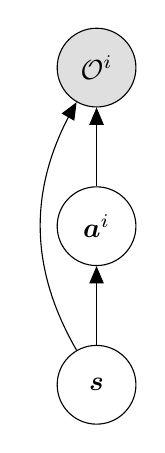
\begin{tikzpicture}[latent/.append style={minimum size=1.0cm}]
        \node[obs] (o) {$\mathcal{O}^i$};
        \node[latent, below=of o] (a) {$\boldsymbol{a}^i$};
        \node[latent, below=of a] (s) {$\boldsymbol{s}$};
    
        \edge {s} {a}
        \edge {a} {o}
        \path[->]  (s)  edge   [bend left=30] node {} (o);
    \end{tikzpicture}
    \end{minipage}%
    \begin{minipage}[t]{0.5\linewidth}
    \captionof{figure}{Graphical model of One-Step Single agent reinforcement learning with visible optimality variable.} 
    \label{fig:one-step-single agent}
    \end{minipage}
\end{figure}
Which in this case, we can arrived at the same objective. However, for multi-agent case, strictly speaking, having difference Lagrange multiplier for each of KL-Divergence term (agent and its opponent) is \emph{impossible} (currently) if we derived the objective from this innocent looking graphical model (see \ref{fig:sad-graphical-balance-q}): 

\begin{figure}[ht]
    \begin{minipage}[t]{0.5\linewidth}
    \centering
    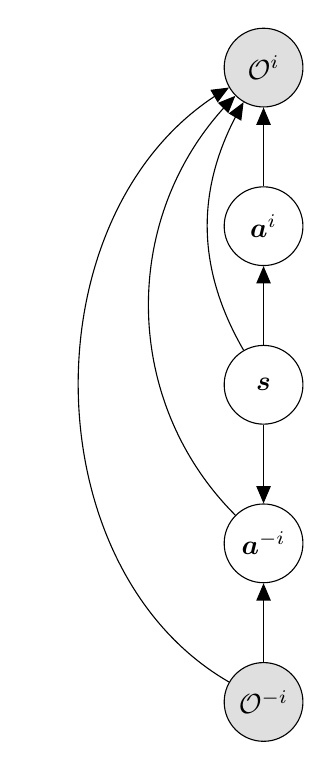
\begin{tikzpicture}[latent/.append style={minimum size=1.0cm}]
        \node[obs] (o) {$\mathcal{O}^i$};
        \node[latent, below=of o] (a) {$\boldsymbol{a}^i$};
        \node[latent, below=of a] (s) {$\boldsymbol{s}$};
        \node[latent, below=of s] (a1) {$\boldsymbol{a}^{-i}$};
        \node[obs, below=of a1] (o1) {$\mathcal{O}^{-i}$};
        
        \edge{o1} {a1}
        \edge {s} {a, a1}
        \edge {a} {o}
        \path[->]  (o1)  edge   [bend left=60] node {} (o);
        \path[->]  (a1)  edge   [bend left=45] node {} (o);
        \path[->]  (s)  edge   [bend left=30] node {} (o);
    \end{tikzpicture}
    \end{minipage}%
    \begin{minipage}[t]{0.5\linewidth}
    \captionof{figure}{An attempts to define Balancing Soft-Q learning via graphical model. We can see that the optimality of the agent $\mathcal{O}^{i}$ is based on the optionally of other agents $\mathcal{O}^{-i}$. Furthermore, the action of opponent agents is assumed to be optimal.} 
    \label{fig:sad-graphical-balance-q}
    \end{minipage}
\end{figure}
Let's first define the joint probability of this graphical model 
\begin{equation}
    \begin{aligned}
        P(\mathcal{O}^i = 1, \boldsymbol{a}^i, \boldsymbol{s}, \boldsymbol{a}^{-i}, \mathcal{O}^{-i} = 1) = &P(\mathcal{O}^i = 1 | \boldsymbol{a}^i, \boldsymbol{s}, \boldsymbol{a}^{-i}, \mathcal{O}^{-i} = 1) \\
        &P_{\text{prior}}(\boldsymbol{a}^i | \boldsymbol{s}) P(\boldsymbol{s}) P_{\text{prior}}(\boldsymbol{a}^{-i} | \boldsymbol{s}, \mathcal{O}^{-i} = 1) P(\mathcal{O}^{-i} = 1)
    \end{aligned}
\end{equation}
Now define the variational distribution. 
\begin{equation}
    \begin{aligned}
        q(\boldsymbol{a}^i, \boldsymbol{s}, \boldsymbol{a}^{-i}, \mathcal{O}^{-i} = 1) = \pi_{\theta} (\boldsymbol{a}^i | \boldsymbol{s}) \rho_{\phi}(\boldsymbol{a}^{-i} | \boldsymbol{s}, \mathcal{O}^{-i} = 1) P(\boldsymbol{s}) P(\mathcal{O}^{-i} = 1)
    \end{aligned}
\end{equation}
Let the optimality of the agent be defined, given that the opponent is optimal to be  
\begin{equation}
    P(\mathcal{O}^i = 1 | \boldsymbol{a}^i, \boldsymbol{s}, \boldsymbol{a}^{-i}, \mathcal{O}^{-i} = 1) = \exp\Big( \beta R(\boldsymbol{s}, \boldsymbol{a}^i, \boldsymbol{a}^{-i}) \Big)
\end{equation}
Now we can see where the variable $\beta$ is coming from. Let's proceed. With this, the ELBO can be found by minimizing KL-Divergence between variational distribution and joint probability:
\begin{equation*}
    \begin{aligned}
        &\begin{aligned}[t]
            \mathbb{E}_{q(\boldsymbol{a}^i, \boldsymbol{s}, \boldsymbol{a}^{-i}, \mathcal{O}^{-i} = 1)} \bigg[ &\log \pi_{\theta} (\boldsymbol{a}^i | \boldsymbol{s}) + \log \rho_{\phi}(\boldsymbol{a}^{-i} | \boldsymbol{s}, \mathcal{O}^{-i} = 1) + \cancel{\log P(\boldsymbol{s})} + \cancel{\log P(\mathcal{O}^{-i} = 1)}  \\
            &-\log \exp\Big( \beta R(\boldsymbol{s}, \boldsymbol{a}^i, \boldsymbol{a}^{-i}) \Big) - \log P_{\text{prior}}(\boldsymbol{a}^i | \boldsymbol{s}) - \cancel{\log  P(\boldsymbol{s})} \\
            &- \log P_{\text{prior}}(\boldsymbol{a}^{-i} | \boldsymbol{s}, \mathcal{O}^{-i} = 1) -\log \cancel{P(\mathcal{O}^{-i} = 1)} \bigg]
        \end{aligned} \\
        &= \begin{aligned}[t]
            \mathbb{E}_{q(\boldsymbol{a}^i, \boldsymbol{s}, \boldsymbol{a}^{-i}, \mathcal{O}^{-i} = 1)} \bigg[ &- \beta R(\boldsymbol{s}, \boldsymbol{a}^i, \boldsymbol{a}^{-i}) + \log \pi_{\theta} (\boldsymbol{a}^i | \boldsymbol{s}) + \log \rho_{\phi}(\boldsymbol{a}^{-i} | \boldsymbol{s}) \\
            &-\log P_{\text{prior}}(\boldsymbol{a}^i | \boldsymbol{s}) - \log P_{\text{prior}}(\boldsymbol{a}^{-i} | \boldsymbol{s}, \mathcal{O}^{-i} = 1) \bigg]
        \end{aligned}
    \end{aligned}
\end{equation*}
This can be seen as maximizing of the following objective 
\begin{equation}
    \mathbb{E}_{q(\boldsymbol{a}^i, \boldsymbol{s}, \boldsymbol{a}^{-i}, \mathcal{O}^{-i} = 1)} \bigg[ R(\boldsymbol{s}, \boldsymbol{a}^i, \boldsymbol{a}^{-i}) + \frac{1}{\beta} \log \frac{\pi_{\theta} (\boldsymbol{a}^i | \boldsymbol{s})}{P_{\text{prior}}(\boldsymbol{a}^i | \boldsymbol{s})}  + \frac{1}{\beta} \log \frac{\rho_{\phi}(\boldsymbol{a}^{-i} | \boldsymbol{s})}{P_{\text{prior}}(\boldsymbol{a}^{-i} | \boldsymbol{s}, \mathcal{O}^{-i} = 1)} \bigg]
\end{equation}
Superficially, the objective looks striking similar to Balancing Soft-Q objective, however, the nature of $\beta$ for each KL-divergence are difference.  This leads to an opponent model that resembles the value viewed by the agent, since $\beta$ are the same for both agent's and opponent model. This leads to a main problem we are trying to solve: \textbf{How to inject opponent's characteristic into our graphical model without relying on Lagrange multiplier ?}

\begin{tcolorbox}
\textbf{Lesson 2: } Opponent Characteristic can't be represented in centralized graphical model -- a graphical model that unifying every dependencies from opponent model to agent's policy -- due to difference characteristic of both agent's and opponent's. Balancing Soft-Q works because it contains separate Lagrange multipliers.
\end{tcolorbox}

Furthermore, although Lagrange multiplier's method yields very interesting objective, we didn't see any connection between constrain on KL-Divergence to a behavior of the agent apart from its rationality. This conclusion comes from the same reason KL-Divergence constraints is introduced in first place -- because we want to limit the rationality of agent alone. 

\begin{tcolorbox}
\textbf{Lesson 3: } Lagrange multiplier's method doesn't make a lot of senses (explanation needed) + not extensible, therefore we really need a graphical model to explain this.
\end{tcolorbox}
\emph{\textbf{Note}: Balancing Soft-Q still got other problems, which we explored later.}  

\subsection{Deriving Optimal Policy for Balancing Soft-Q}
Let's see how to derive the optimal policy from the objective. This will be the common pattern, when we derive others algorithms. Finally, this is based on \cite{levine2018reinforcement} message passing, however, considering only the base case. We would like to find the optimal opponent by maximising the following objective with respect to $\rho_{\phi}$ (We also define a normalizing term/message to be $N(\boldsymbol{s}, \boldsymbol{a}^i)$. The real definition will be clear afterward)

\begin{equation*}
    \begin{aligned}
        \mathbb{E}_{q(\boldsymbol{s}, \boldsymbol{a}^i)}&\bigg[ \mathbb{E}_{q(\boldsymbol{a}^{-i} | \boldsymbol{s})} \bigg[ R(\boldsymbol{s}, \boldsymbol{a}^i, \boldsymbol{a}^{-i}) - \frac{1}{\beta_{-i}}\log \frac{\rho_{\phi}(\boldsymbol{a}^i | \boldsymbol{s})}{P_{\text{prior}}(\boldsymbol{a}^{-i} | \boldsymbol{s})}  \bigg] - \frac{1}{\beta_{i}}\log \frac{\pi_{\theta}(\boldsymbol{a}^i | \boldsymbol{s})}{P_{\text{prior}}(\boldsymbol{a}^i | \boldsymbol{s})} \bigg] \\
        &= \begin{aligned}[t]
            \mathbb{E}_{q(\boldsymbol{s}, \boldsymbol{a}^i)} \bigg[ \mathbb{E}_{q(\boldsymbol{a}^{-i} | \boldsymbol{s})} \bigg[ R&(\boldsymbol{s}, \boldsymbol{a}^i, \boldsymbol{a}^{-i}) - \frac{1}{\beta_{-i}}\log \rho_{\phi}(\boldsymbol{a}^i | \boldsymbol{s})  \\
            &+\frac{1}{\beta_{-i}} \log P_{\text{prior}}(\boldsymbol{a}^{-i} | \boldsymbol{s}) - N(\boldsymbol{s}, \boldsymbol{a}^{i}) + N(\boldsymbol{s}, \boldsymbol{a}^{i}) \bigg] \\
            &+\frac{1}{\beta_{i}}\log \frac{\pi_{\theta}(\boldsymbol{a}^i | \boldsymbol{s})}{P_{\text{prior}}(\boldsymbol{a}^i | \boldsymbol{s})} \bigg]
        \end{aligned} \\
        &= \begin{aligned}[t]
            \mathbb{E}_{q(\boldsymbol{s}, \boldsymbol{a}^i, \boldsymbol{a}^{-i})}[N(\boldsymbol{s}, \boldsymbol{a}^i)] - \mathbb{E}_{q(\boldsymbol{s}, \boldsymbol{a}^i)} \bigg[ \mathbb{E}_{q(\boldsymbol{a}^{-i} | \boldsymbol{s})} \bigg[ -R&(\boldsymbol{s}, \boldsymbol{a}^i, \boldsymbol{a}^{-i}) + \frac{1}{\beta_{-i}}\log \rho_{\phi}(\boldsymbol{a}^i | \boldsymbol{s})  \\
            &-\frac{1}{\beta_{-i}} \log P_{\text{prior}}(\boldsymbol{a}^{-i} | \boldsymbol{s})+ N(\boldsymbol{s}, \boldsymbol{a}^{i}) \bigg] \\
            &+\frac{1}{\beta_{i}}\log \frac{\pi_{\theta}(\boldsymbol{a}^i | \boldsymbol{s})}{P_{\text{prior}}(\boldsymbol{a}^i | \boldsymbol{s})}\bigg]
        \end{aligned} \\
        &= \begin{aligned}[t]
            \mathbb{E}_{q(\boldsymbol{s}, \boldsymbol{a}^i, \boldsymbol{a}^{-i})}[N(\boldsymbol{s}, \boldsymbol{a}^i)] - \mathbb{E}_{q(\boldsymbol{s}, \boldsymbol{a}^i)} \bigg[ \mathbb{E}_{q(\boldsymbol{a}^{-i} | \boldsymbol{s})} \bigg[ -\beta_{-i} R&(\boldsymbol{s}, \boldsymbol{a}^i, \boldsymbol{a}^{-i}) + \log \rho_{\phi}(\boldsymbol{a}^i | \boldsymbol{s})  \\
            &-\log P_{\text{prior}}(\boldsymbol{a}^{-i} | \boldsymbol{s})+ N(\boldsymbol{s}, \boldsymbol{a}^{i}) \bigg] \\
            &+\frac{\beta_{-i}}{\beta_{i}}\log \frac{\pi_{\theta}(\boldsymbol{a}^i | \boldsymbol{s})}{P_{\text{prior}}(\boldsymbol{a}^i | \boldsymbol{s})}\bigg]
        \end{aligned}  \\
        &= \begin{aligned}[t]
            \mathbb{E}_{q(\boldsymbol{s}, \boldsymbol{a}^i, \boldsymbol{a}^{-i})}[N(\boldsymbol{s}, \boldsymbol{a}^i)] - \mathbb{E}_{q(\boldsymbol{s}, \boldsymbol{a}^i)} \bigg[ \mathbb{E}_{q(\boldsymbol{a}^{-i} | \boldsymbol{s})} \bigg[ &\log \rho_{\phi}(\boldsymbol{a}^i | \boldsymbol{s}) \\
            &-\bigg[ \beta_{-i} R(\boldsymbol{s}, \boldsymbol{a}^i, \boldsymbol{a}^{-i})   +\log P_{\text{prior}}(\boldsymbol{a}^{-i} | \boldsymbol{s}) - 
            N(\boldsymbol{s}, \boldsymbol{a}^{i}) \bigg] \bigg] \\
            &+\frac{\beta_{-i}}{\beta_{i}}\log \frac{\pi_{\theta}(\boldsymbol{a}^i | \boldsymbol{s})}{P_{\text{prior}}(\boldsymbol{a}^i | \boldsymbol{s})}\bigg]
        \end{aligned} \\
        &= \begin{aligned}[t]
            \mathbb{E}_{q(\boldsymbol{s}, \boldsymbol{a}^i, \boldsymbol{a}^{-i})}[ N(\boldsymbol{s}, \boldsymbol{a}^i)] - \mathbb{E}_{q(\boldsymbol{s}, \boldsymbol{a}^i)} \Bigg[ &D_{KL}\Bigg[ \rho_{\phi}(\boldsymbol{a}^i | \boldsymbol{s}) \Bigg|\Bigg| \frac{\exp(\beta_{-i} R(\boldsymbol{s}, \boldsymbol{a}^i, \boldsymbol{a}^{-i}))P_{\text{prior}}(\boldsymbol{a}^{-i} | \boldsymbol{s})}{\exp N(\boldsymbol{s}, \boldsymbol{a}^{i})} \Bigg] \Bigg] \\  &+\frac{\beta_{-i}}{\beta_{i}}\log \frac{\pi_{\theta}(\boldsymbol{a}^i | \boldsymbol{s})}{P_{\text{prior}}(\boldsymbol{a}^i | \boldsymbol{s})}\bigg]
        \end{aligned} 
    \end{aligned}
\end{equation*}
\textbf{Note: } We absolve the constant $\beta_{-i}$ inside the normalizing factor. The optimal opponent is then equal to (There is a problem with $\boldsymbol{a}^i$. However, we care about using its policy to find the final value.)
\begin{equation}
    \rho_{\phi}(\boldsymbol{a}^{-i} | \boldsymbol{s}) = \frac{\exp(\beta_{-i} R(\boldsymbol{s}, \boldsymbol{a}^i, \boldsymbol{a}^{-i}))P_{\text{prior}}(\boldsymbol{a}^{-i} | \boldsymbol{s})}{\exp N(\boldsymbol{s}, \boldsymbol{a}^{i})}
\end{equation}
This also leads to a normalizing factor of 
\begin{equation}
    N(\boldsymbol{s}, \boldsymbol{a}^{i}) = \frac{1}{\beta_{-i} }\log \int_{\mathcal{A}^{-i}} \exp(R(\boldsymbol{s}, \boldsymbol{a}^i, \boldsymbol{a}^{-i}))P_{\text{prior}}(\boldsymbol{a}^{-i} | \boldsymbol{s})
\end{equation}
We can interpret this as agent's Q-value function based on prior knowledge of opponent \cite{grau2018balancing}. After getting the optimal opponent that is solely based on $R(\boldsymbol{s}, \boldsymbol{a}, \boldsymbol{a}^{-i})$, now we can find the agent optimal policy by substitute this optimal opponent back, and optimize the agent's policy instead.

\begin{equation*}
    \begin{aligned}
        &\mathbb{E}_{q(\boldsymbol{s}, \boldsymbol{a}^i, \boldsymbol{a}^{-i})}\bigg[ R(\boldsymbol{s}, \boldsymbol{a}^i, \boldsymbol{a}^{-i})  - \frac{1}{\beta_{i}}\log \frac{\pi_{\theta}(\boldsymbol{a}^i | \boldsymbol{s})}{P_{\text{prior}}(\boldsymbol{a}^i | \boldsymbol{s})}  - \frac{1}{\beta_{-i}}\log \frac{\exp(\beta_{-i} R(\boldsymbol{s}, \boldsymbol{a}^i, \boldsymbol{a}^{-i}))\cancel{P_{\text{prior}}(\boldsymbol{a}^{-i} | \boldsymbol{s})}}{\exp  N(\boldsymbol{s}, \boldsymbol{a}^{i}) \cancel{P_{\text{prior}}(\boldsymbol{a}^{-i} | \boldsymbol{s})} } \bigg] \\
        &= \mathbb{E}_{q(\boldsymbol{s}, \boldsymbol{a}^i, \boldsymbol{a}^{-i})}\bigg[ \cancel{R(\boldsymbol{s}, \boldsymbol{a}^i, \boldsymbol{a}^{-i})}  - \frac{1}{\beta_{i}}\log \frac{\pi_{\theta}(\boldsymbol{a}^i | \boldsymbol{s})}{P_{\text{prior}}(\boldsymbol{a}^i | \boldsymbol{s})}  - \cancel{R(\boldsymbol{s}, \boldsymbol{a}^i, \boldsymbol{a}^{-i}))} + \underbrace{ \frac{1}{\beta_{-i}}\log \exp N(\boldsymbol{s}, \boldsymbol{a}^{i})}_{R(\boldsymbol{s}, \boldsymbol{a}^i)} \bigg]\\
        &= \mathbb{E}_{q(\boldsymbol{s}, \boldsymbol{a}^i, \boldsymbol{a}^{-i})}\bigg[ \beta_i R(\boldsymbol{s}, \boldsymbol{a}^i) - \log \pi_{\theta}(\boldsymbol{a}^i | \boldsymbol{s}) +  P_{\text{prior}}(\boldsymbol{a}^i | \boldsymbol{s}) + N(\boldsymbol{s}) - N(\boldsymbol{s}) \bigg] \\
        &= \mathbb{E}_{q(\boldsymbol{s}, \boldsymbol{a}^i, \boldsymbol{a}^{-i})}[N(\boldsymbol{s})] - 
        \mathbb{E}_{q(\boldsymbol{s}, \boldsymbol{a}^i, \boldsymbol{a}^{-i})}\bigg[ -\beta_i R(\boldsymbol{s}, \boldsymbol{a}^i) + \log \pi_{\theta}(\boldsymbol{a}^i | \boldsymbol{s}) -  P_{\text{prior}}(\boldsymbol{a}^i | \boldsymbol{s}) + N(\boldsymbol{s}) \bigg] \\
        &= \mathbb{E}_{q(\boldsymbol{s}, \boldsymbol{a}^i, \boldsymbol{a}^{-i})}[N(\boldsymbol{s})] - 
        \mathbb{E}_{q(\boldsymbol{s}, \boldsymbol{a}^i, \boldsymbol{a}^{-i})}\bigg[\log \pi_{\theta}(\boldsymbol{a}^i | \boldsymbol{s}) - \bigg[\beta_i R(\boldsymbol{s}, \boldsymbol{a}^i) +P_{\text{prior}}(\boldsymbol{a}^i | \boldsymbol{s}) -  N(\boldsymbol{s}) \bigg] \bigg] \\
        &= \mathbb{E}_{q(\boldsymbol{s}, \boldsymbol{a}^i \boldsymbol{a}^{-i})}[N(\boldsymbol{s})] - 
        \mathbb{E}_{q(\boldsymbol{s},  \boldsymbol{a}^{-i})}\bigg[D_{KL}\bigg[ \log \pi_{\theta}(\boldsymbol{a}^i | \boldsymbol{s}) \bigg|\bigg| \frac{\exp\left( \beta_i R(\boldsymbol{s}, \boldsymbol{a}^i)\right) P_{\text{prior}}(\boldsymbol{a}^i | \boldsymbol{s})}{N(\boldsymbol{s})}  \bigg]\bigg]
    \end{aligned} 
\end{equation*}
In order to max the objective we have to set $\pi_{\theta}$ to be equal to 

\begin{equation*}
    \pi_{\theta}(\boldsymbol{a}^i | \boldsymbol{s}) = \frac{\exp\left( \beta_i R(\boldsymbol{s}, \boldsymbol{a}^i)\right) P_{\text{prior}}(\boldsymbol{a}^i | \boldsymbol{s})}{N(\boldsymbol{s})}
\end{equation*}
This corresponds directly to \cite{grau2018balancing} optimal policy. However, if we can see, the term $R(\boldsymbol{s}, \boldsymbol{a}^i, \boldsymbol{a}^{-i})$ got cancelled due to the Lagrange multiplier on $\log \frac{\rho_{\phi}(\boldsymbol{a}^i | \boldsymbol{s})}{P_{\text{prior}}(\boldsymbol{a}^{-i} | \boldsymbol{s})}$. With this observation and our derivation of Balancing Soft-Q, we can conclude that: 

\begin{tcolorbox}
\textbf{Lesson 4: }\label{lesson:4} We need to have an \textbf{independent inference method for calculating opponent's model} (if we want to do it in decentralized version). \cite{grau2018balancing} works can be seen as non-decentralized version of ROMMEO (since we directly use \textit{opponent's optimal policy against agent's prior or simply ignore it} the agent's policy should be $\pi(\boldsymbol{a}^i | \boldsymbol{s}, \boldsymbol{a}^{-i})$)
\end{tcolorbox}

\begin{tcolorbox}
\textbf{Lesson 5: } There are 2 steps we have to make: first finding the extream case of the value function, then we can find a policy.  
\end{tcolorbox}

\section{Unified View}
\subsection{Attempts to split}
Let's start with a graphical model. Since we are going to split the worlds, we will first find an optimal $\pi(\boldsymbol{a}^i | \boldsymbol{s}, \boldsymbol{a}^{-i})$ Playing against an opponent, which may or may not be optimal. Noted that $\mathcal{O}^{-i}$ isn't necessary since locally, given the opponent policy, the most optimal thing is to maximizes its own reward.
\textbf{BETTER with FACTORED Graph}

\begin{figure}[t]
    \begin{minipage}[t]{0.5\linewidth}
    \centering
    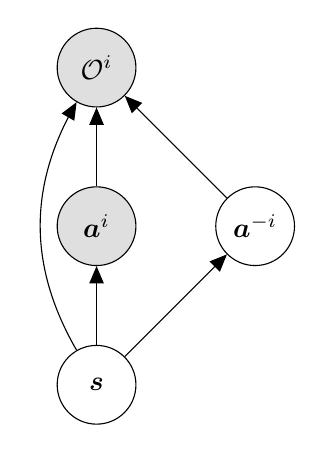
\begin{tikzpicture}[latent/.append style={minimum size=1.0cm}]
        \node[obs] (o) {$\mathcal{O}^i$};
        \node[obs, below=of o] (a) {$\boldsymbol{a}^i$};
        \node[latent, below=of a] (s) {$\boldsymbol{s}$};
        \node[latent, right=of a] (a1) {$\boldsymbol{a}^{-i}$};
        % \node[latent, right=2.3cm of o] (o1) {$\mathcal{O}^{-i}$};
        
        % above right=1.3cm of a
        
        \edge {s} {a, a1}
        \edge {a} {o}
        % \edge {o1} {o, a1}
        % \edge {a1} {a}
        \edge {a1} {o}
        \path[->]  (s)  edge   [bend left=30] node {} (o);
    \end{tikzpicture}
    \end{minipage}%
    \begin{minipage}[t]{0.5\linewidth}
    \captionof{figure}{Graphical model of splitted graphical model for agent's policy. } 
    % \label{fig:}
    \end{minipage}
\end{figure}
Start with finding the joint probability of the graphical model.
\begin{equation}
    P_{\text{prior}}(\boldsymbol{a}^{-i} | \boldsymbol{s}) P_{\text{prior}}(\boldsymbol{a}^i | \boldsymbol{s}, \boldsymbol{a}^{-i}) P(\boldsymbol{s}) P(\mathcal{O}^i = 1 | \boldsymbol{s}, \boldsymbol{a}^i, \boldsymbol{a}^{-i})
\end{equation}
We can see that the variational distribution can be defined as: (assuming that the )
\begin{equation}
    P_{\text{prior}}(\boldsymbol{a}^{-i} | \boldsymbol{s}) \pi_{\theta}(\boldsymbol{a}^{i} | \boldsymbol{s}, \boldsymbol{a}^{-i}) P(\boldsymbol{s})
\end{equation}
Then the approximate variational inference can be done by minimising the KL-Divergence, hence, we have the following objective 

\begin{equation}
    \begin{aligned}
        &\begin{aligned}
            \mathbb{E}_{q(\boldsymbol{a}^{i}, \boldsymbol{a}^{-i}, \boldsymbol{s})}\bigg[&\cancel{\log P_{\text{prior}}(\boldsymbol{a}^{-i} | \boldsymbol{s})} + \log \pi_{\theta}(\boldsymbol{a}^{i} | \boldsymbol{s}, \boldsymbol{a}^{-i}) + \log \cancel{P(\boldsymbol{s})} - \log P_{\text{prior}}(\boldsymbol{a}^{i} | \boldsymbol{s}, \boldsymbol{a}^{-i}) \\
            &- \cancel{\log P_{\text{prior}}(\boldsymbol{a}^{-i} | \boldsymbol{s})} - \cancel{\log P(\boldsymbol{s})} -\log P(\mathcal{O}^i = 1 | \boldsymbol{s}, \boldsymbol{a}^i, \boldsymbol{a}^{-i}) \bigg]
        \end{aligned} \\ 
        &= \mathbb{E}_{q(\boldsymbol{a}^{i}, \boldsymbol{a}^{-i}, \boldsymbol{s})}\bigg[ -\beta_i R(\boldsymbol{s}, \boldsymbol{a}^i, \boldsymbol{a}^{-i}) + \log \frac{\pi_{\theta}(\boldsymbol{a}^{i} | \boldsymbol{s},\boldsymbol{a}^{-i})}{P_{\text{prior}}(\boldsymbol{a}^{-i} | \boldsymbol{s}, \boldsymbol{a}^{-i})} \bigg] \\ 
    \end{aligned}
\end{equation}
This is equal to maximizing the following objective 
\begin{equation}
    \mathbb{E}_{q(\boldsymbol{a}^{i}, \boldsymbol{a}^{-i}, \boldsymbol{s})}\bigg[\beta_i R(\boldsymbol{s}, \boldsymbol{a}^i, \boldsymbol{a}^{-i}) - \log \frac{\pi_{\theta}(\boldsymbol{a}^{i} | \boldsymbol{s},\boldsymbol{a}^{-i})}{P_{\text{prior}}(\boldsymbol{a}^{-i} | \boldsymbol{s}, \boldsymbol{a}^{-i})} \bigg]
\end{equation}
We can find the solution in a closed form by having 
\begin{equation}
    \begin{aligned}
        &\mathbb{E}_{q(\boldsymbol{a}^{i}, \boldsymbol{a}^{-i}, \boldsymbol{s})}\bigg[\beta_i R(\boldsymbol{s}, \boldsymbol{a}^i, \boldsymbol{a}^{-i}) - \log \frac{\pi_{\theta}(\boldsymbol{a}^{i} | \boldsymbol{s},\boldsymbol{a}^{-i})}{P_{\text{prior}}(\boldsymbol{a}^{i} | \boldsymbol{s}, \boldsymbol{a}^{-i})} + N^{i}(\boldsymbol{s}, \boldsymbol{a}^{-i}) - N^{i}(\boldsymbol{s}, \boldsymbol{a}^{-i}) \bigg] \\
        & = \begin{aligned}[t]
            \mathbb{E}_{q(\boldsymbol{a}^{i}, \boldsymbol{a}^{-i}, \boldsymbol{s})}&\bigg[ N^{i}(\boldsymbol{s}, \boldsymbol{a}^{-i}) \bigg] - \mathbb{E}_{q(\boldsymbol{a}^{i}, \boldsymbol{a}^{-i}, \boldsymbol{s})}\bigg[ \log \pi_{\theta}(\boldsymbol{a}^{i} | \boldsymbol{s},\boldsymbol{a}^{-i}) \\
            &- \bigg[ \log \exp\Big(\beta_i R(\boldsymbol{s}, \boldsymbol{a}^i, \boldsymbol{a}^{-i})\Big) - \log \exp N^{i}(\boldsymbol{s}, \boldsymbol{a}^{-i}) + \log P_{\text{prior}}(\boldsymbol{a}^{i} | \boldsymbol{s}, \boldsymbol{a}^{-i})  \bigg] \bigg]
        \end{aligned} \\
        &= \mathbb{E}_{q(\boldsymbol{a}^{i}, \boldsymbol{a}^{-i}, \boldsymbol{s})}\left[ N^{i}(\boldsymbol{s}, \boldsymbol{a}^{-i}) \right] - \mathbb{E}_{q(\boldsymbol{a}^{-i}, \boldsymbol{s})}\left[ D_{KL}\left[ \pi_{\theta}(\boldsymbol{a}^{i} | \boldsymbol{s},\boldsymbol{a}^{-i}) \Bigg|\Bigg| \frac{\exp(\beta_i R(\boldsymbol{s}, \boldsymbol{a}^i, \boldsymbol{a}^{-i})) P_{\text{prior}}(\boldsymbol{a}^{i} | \boldsymbol{s}, \boldsymbol{a}^{-i})}{ \exp N^{i}(\boldsymbol{s}, \boldsymbol{a}^{-i})} \right]\right] 
    \end{aligned}
\end{equation}
We can see that, we can easily see that if want to maximizes the equation, we can set 
\begin{equation}
    \pi_{\theta}(\boldsymbol{a}^{i} | \boldsymbol{s},\boldsymbol{a}^{-i}) = \frac{\exp(\beta_i R(\boldsymbol{s}, \boldsymbol{a}^i, \boldsymbol{a}^{-i})) P_{\text{prior}}(\boldsymbol{a}^{i} | \boldsymbol{s}, \boldsymbol{a}^{-i})}{ \exp N^{i}(\boldsymbol{s}, \boldsymbol{a}^{-i})}
\end{equation}
Where $N^{i}(\boldsymbol{s}, \boldsymbol{a}^{-i})$ can be interpreted as the max expected return of the agent given the current state and opponent action based on agent's prior action.
\begin{equation}
    N^{i}(\boldsymbol{s}, \boldsymbol{a}^{-i}) = \log \int \exp(\beta_i R(\boldsymbol{s}, \boldsymbol{a}^i, \boldsymbol{a}^{-i})) P_{\text{prior}}(\boldsymbol{a}^{i} | \boldsymbol{s}, \boldsymbol{a}^{-i}) \ d\boldsymbol{a}^i
\end{equation}
Since we found a true $\pi_{\theta}(\boldsymbol{a}^{i} | \boldsymbol{s},\boldsymbol{a}^{-i})$ we know that the optimizing objective is left with only $N^{i}(\boldsymbol{s}, \boldsymbol{a}^{-i})$, which we can use in finding optimal opponent's policy. But first, let's define the graphical model for opponent's policy.

\begin{figure}[t]
    \begin{minipage}[t]{0.5\linewidth}
    \centering
    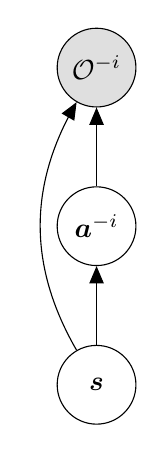
\begin{tikzpicture}[latent/.append style={minimum size=1.0cm}]
        \node[obs] (o) {$\mathcal{O}^{-i}$};
        \node[latent, below=of o] (a1) {$\boldsymbol{a}^{-i}$};
        \node[latent, below=of a1] (s) {$\boldsymbol{s}$};
        % \node[latent, right=2.3cm of o] (o1) {$\mathcal{O}^{-i}$};
        
        % above right=1.3cm of a
        
        \edge {s} {a1}
        % \edge {a} {o}
        % \edge {o1} {o, a1}
        % \edge {a1} {a}
        \edge {a1} {o}
        \path[->]  (s)  edge   [bend left=30] node {} (o);
    \end{tikzpicture}
    \end{minipage}%
    \begin{minipage}[t]{0.5\linewidth}
    \captionof{figure}{Graphical model of splitted graphical model for opponent's policy. } 
    % \label{fig:}
    \end{minipage}
\end{figure}

Surprisingly, the opponent's policy optimality can be defined to be 
\begin{equation}
    P(\mathcal{O}^{-i} = 1 | \boldsymbol{s}, \boldsymbol{a}^{-i}) = \exp(\beta_{-i} N^{i}(\boldsymbol{s}, \boldsymbol{a}^{-i}))
\end{equation}
This can be justified in 2 ways 
\begin{itemize}
    \item This is based on \cite{grau2018balancing}, where it states that in action selection for the opponent model (in this case), "depends on the action of the our actor(other agent), which is unknown a priori". Strictly speaking, this is also based on the $\arg\max\text{ext}$ of value function (what we have left from maximizing agent's return from previous graphical model). 
    \item Having $\beta_i$ implies that the characteristic of the opponent model is based on the soft-maximum of agent's return. (aka. best at what prior agent can do) If $\beta_{-i}$ is negative then the selection of the action will be the one that would make the agent's return smallest and vice versa. Furthermore, having small $\beta_{-i}$ leads to policy that should be near the opponent model's prior.
\end{itemize}
With this, we can define the joint distribution to be 
\begin{equation}
    P(\boldsymbol{s}) P_{\text{prior}}(\boldsymbol{a}^{-i} | \boldsymbol{s}) P(\mathcal{O}^{-i} = 1 | \boldsymbol{s}, \boldsymbol{a}^{-i})
\end{equation}
The variational distribution is 
\begin{equation}
    P(\boldsymbol{s}) \rho_{\phi}(\boldsymbol{a}^{-i} | \boldsymbol{s})
\end{equation}
Finally, we can set 
\begin{equation}
    \rho_{\phi}(\boldsymbol{a}^{-i} | \boldsymbol{s}) = \frac{\exp(\beta_{-i} N(\boldsymbol{s}, \boldsymbol{a}^{-i})) P_{\text{prior}}(\boldsymbol{a}^{-i} | \boldsymbol{s})}{\exp N(\boldsymbol{s})}
\end{equation}
where 
\begin{equation}
    N(\boldsymbol{s}) = \log \int_{\mathcal{A}^{-i}} \exp(\beta_{-i} N(\boldsymbol{s}, \boldsymbol{a}^{-i})) P_{\text{prior}}(\boldsymbol{a}^{-i} | \boldsymbol{s})
\end{equation}
We can show that ROMMEO with the following objective 
\begin{equation}
    \mathbb{E}\Bigg[ R(\boldsymbol{s}, \boldsymbol{a}^i, \boldsymbol{a}^{-i}) - \frac{1}{\beta_i} \log \frac{\pi_{\theta}(\boldsymbol{a}^i | \boldsymbol{s}, \boldsymbol{a}^{-i})}{P_{\text{prior}}(\boldsymbol{a}^i | \boldsymbol{s}, \boldsymbol{a}^{-i})} - \frac{1}{\beta_{-i}} \log \frac{\rho_{\phi}(\boldsymbol{a}^{-i} | \boldsymbol{s})}{P_{\text{prior}}(\boldsymbol{a}^{-i} | \boldsymbol{s})}  \Bigg]
\end{equation}
Yields the same result. Thus, we have ROMMEO that works for both zero-sum game and team game, represented in a separates graphical model. 
% \subsection{ROMMEO with Balanced-Q}

% \begin{equation}
%     \mathbb{E}_{q(\boldsymbol{s}, \boldsymbol{a}^{-i}, \boldsymbol{a}^{-i})}
% \end{equation}


















% \section{Unified View}
% \subsection{Single-Step Balancing Soft-Q \cite{grau2018balancing} with ROMMEO \cite{tian2019regularized}}
% \subsection{Single-Step PR2 \cite{wen2019probabilistic}}
% \subsection{Single-Step GR2 \cite{wen2019multi}}

% \section{Additional Features}
% \subsection{Belief Over Agent's Characteristic}
% \subsection{Extension to General Sum Game}




% We will start by formalizing difference graphical models representing our assumptions on agents and their interaction. This will lead to ELBO representing methods in difference literature including:  \cite{tian2019regularized}, \cite{grau2018balancing}, and \cite{wen2019probabilistic}. Furthermore, we will extend this framework to new objective function. Let's start with one-step game, and extending to stochastic game can be shown to be arbitrary.

\section{Single-Step ROMMEO \cite{tian2019regularized}}

This is based on the perspective of agent $i$.

\begin{figure}[ht]
    \begin{minipage}[t]{0.5\linewidth}
    \centering
    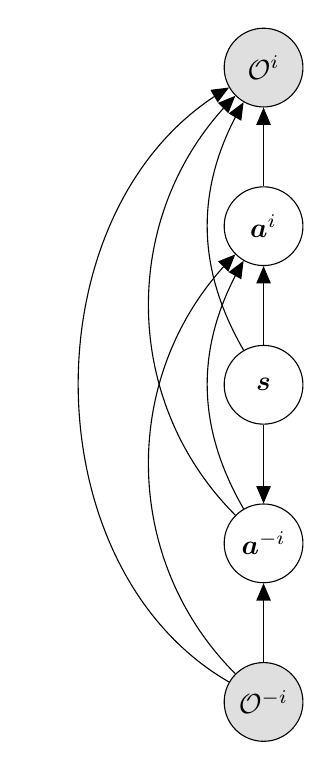
\begin{tikzpicture}[latent/.append style={minimum size=1.0cm}]
        \node[obs] (o) {$\mathcal{O}^i$};
        \node[latent, below=of o] (a) {$\boldsymbol{a}^i$};
        \node[latent, below=of a] (s) {$\boldsymbol{s}$};
        \node[latent, below=of s] (a1) {$\boldsymbol{a}^{-i}$};
        \node[obs, below=of a1] (o1) {$\mathcal{O}^{-i}$};
        
        
        \path[->]  (o1)  edge   [bend left=45] node {} (a);
        \edge{o1} {a1}
        \edge {s} {a, a1}
        \edge {a} {o}
        \path[->]  (o1)  edge   [bend left=60] node {} (o);
        \path[->]  (a1)  edge   [bend left=45] node {} (o);
        \path[->]  (a1)  edge   [bend left=30] node {} (a);
        \path[->]  (s)  edge   [bend left=30] node {} (o);
    \end{tikzpicture}
    \label{ROMMEO-Graphical}
    \end{minipage}%
    \begin{minipage}[t]{0.5\linewidth}
    Graphical model of One-Step ROMMEO \cite{tian2019regularized}. We can see that the optimality of the agent $\mathcal{O}^{i}$ is based on the optionally of other agents $\mathcal{O}^{-i}$. Furthermore, the action of opponent agents is assumed to be optimal.
    \end{minipage}
\end{figure}

% \begin{figure}[!h]
 
% \end{figure}
Assuming the opponent model is \emph{Optimal} i.e $P(\mathcal{O}^{-i} = 1) = 1$ As we would like to find the variational distribution $q(\boldsymbol{s}, \boldsymbol{a}^i, \boldsymbol{a}^{-i} | \mathcal{O}^{-i} = 1)$, which can be represented (factorized) as 

\begin{equation}
    q(\boldsymbol{s}, \boldsymbol{a}^i, \boldsymbol{a}^{-i} | \mathcal{O}^{-i} = 1) = \pi_{\theta}(\boldsymbol{a}^i | \boldsymbol{s}, \boldsymbol{a}^{-i}) \cdot \rho_{\phi}(\boldsymbol{a}^{-i} | \boldsymbol{s}, \mathcal{O}^{-i} = 1) \cdot P(\boldsymbol{s})
\end{equation}
This implies that ELBO can be found by minimizing the KL-Divergence between $q(\boldsymbol{s}, \boldsymbol{a}^i, \boldsymbol{a}^{-i} | \mathcal{O}^{-i} = 1)$ and $P(\boldsymbol{s}, \boldsymbol{a}^i, \boldsymbol{a}^{-i} | \mathcal{O}^{i} = \mathcal{O}^{-i} = 1)$, where (The joint distribution factorization following \ref{ROMMEO-Graphical})

\begin{equation}
    \begin{aligned}
        P(\boldsymbol{s}, \boldsymbol{a}, \boldsymbol{a}^{-i} | \mathcal{O}^{i} = \mathcal{O}^{-i} = 1) &= \frac{P(\boldsymbol{s}, \boldsymbol{a}^i, \boldsymbol{a}^{-i}, \mathcal{O}^{i} = 1,  \mathcal{O}^{-i} = 1)}{\int P(\boldsymbol{s}, \boldsymbol{a}^i, \boldsymbol{a}^{-i}, \mathcal{O}^{i} = 1,  \mathcal{O}^{-i} = 1) \ d\boldsymbol{s} \ d\boldsymbol{a}^i \ d\boldsymbol{a}^{-i}} \\ 
        &\propto \begin{aligned}[t]
            &P(\mathcal{O}^i = 1 | \boldsymbol{s}, \boldsymbol{a}^i, \boldsymbol{a}^{-i}, \mathcal{O}^{-i} = 1) \cdot P_{\text{prior}}(\boldsymbol{a}^i | \boldsymbol{s}, \boldsymbol{a}^{-i}, \mathcal{O}^{-i} = 1) \cdot \\
            &P(\boldsymbol{s}) \cdot P(\boldsymbol{a}^{-i} |\boldsymbol{s}, \mathcal{O}^{-i} = 1) \cdot P(\mathcal{O}^{i})
        \end{aligned}
    \end{aligned}
\end{equation}

In \cite{tian2019regularized}, the game is assumed to be fully cooperative game, meaning that we can define the optimality of agent $it$ to be (with respect to opponent being optimal)

\begin{equation}
    P(\mathcal{O}^i = 1 | \boldsymbol{s}, \boldsymbol{a}^i, \boldsymbol{a}^{-i}, \mathcal{O}^{-i} = 1) \propto \exp \left( \beta R(\boldsymbol{s}, \boldsymbol{a}^i, \boldsymbol{a}^{-i}) \right)
\end{equation}
By finding the KL-Divergence between variational distribution and posterior, we have 

\begin{equation}
    \begin{aligned}
        \mathbb{E}_{(\boldsymbol{s}, \boldsymbol{a}^i, \boldsymbol{a}^{-i}) \sim q(\boldsymbol{s}, \boldsymbol{a}^i, \boldsymbol{a}^{-i} | \mathcal{O}^{-i} = 1)} &\Big[\log q(\boldsymbol{s}, \boldsymbol{a}^i, \boldsymbol{a}^{-i} | \mathcal{O}^{-i} = 1) - \log P(\boldsymbol{s}, \boldsymbol{a}, \boldsymbol{a}^{-i} | \mathcal{O}^{i} = \mathcal{O}^{-i} = 1) \Big] \\
        &= \begin{aligned}[t]
                \mathbb{E}\Big[ \log \pi_{\theta}(\boldsymbol{a}^i | \boldsymbol{s}, \boldsymbol{a}^{-i}) &+ \log \rho_{\phi}(\boldsymbol{a}^{-i} | \boldsymbol{s}, \mathcal{O}^{-i} = 1) + \cancel{\log P(\boldsymbol{s})} \\
                &-\log P(\mathcal{O}^i = 1 | \boldsymbol{s}, \boldsymbol{a}^i, \boldsymbol{a}^{-i}, \mathcal{O}^{-i} = 1) \\
                &- \log P_{\text{prior}}(\boldsymbol{a}^i | \boldsymbol{s}, \boldsymbol{a}^{-i}, \mathcal{O}^{-i} = 1) - \cancel{\log P(\boldsymbol{s})} \\
                &- \log P(\boldsymbol{a}^{-i} |\boldsymbol{s}, \mathcal{O}^{-i} = 1) - \log P(\mathcal{O}^{i}) \Big] 
            \end{aligned} \\
        &= \begin{aligned}[t]
                &\mathbb{E}\Big[ \log \pi_{\theta}(\boldsymbol{a}^i | \boldsymbol{s}, \boldsymbol{a}^{-i}) -  \log P_{\text{prior}}(\boldsymbol{a}^i | \boldsymbol{s}, \boldsymbol{a}^{-i}, \mathcal{O}^{-i} = 1) \Big] \\ 
                &+\mathbb{E}\Big[ \log \rho_{\phi}(\boldsymbol{a}^{-i} | \boldsymbol{s}, \mathcal{O}^{-i} = 1) - \log P(\boldsymbol{a}^{-i} |\boldsymbol{s}, \mathcal{O}^{-i} = 1) \Big] \\
                &-\beta R(\boldsymbol{s}, \boldsymbol{a}^i, \boldsymbol{a}^{-i}) -\log 1
            \end{aligned}
    \end{aligned} 
\end{equation}
This is equal to maximizing the following objective as defined in \cite{tian2019regularized}, with single step (Where the authors defined $P_{\text{prior}}$ to be uniform distribution over actions)
\begin{equation}
    \begin{aligned}
        \mathbb{E}_{(\boldsymbol{s}, \boldsymbol{a}^i, \boldsymbol{a}^{-i}) \sim q(\boldsymbol{s}, \boldsymbol{a}^i, \boldsymbol{a}^{-i} | \mathcal{O}^{-i} = 1)}\bigg[R(\boldsymbol{s}, \boldsymbol{a}^i, \boldsymbol{a}^{-i}) &- \frac{1}{\beta} D_{KL} \Big(\pi_{\theta}(\boldsymbol{a}^i | \boldsymbol{s}, \boldsymbol{a}^{-i}) \Big|\Big| P_{\text{prior}}(\boldsymbol{a}^i | \boldsymbol{s}, \boldsymbol{a}^{-i}, \mathcal{O}^{-i} = 1) \Big)  \\
        & - \frac{1}{\beta} D_{KL} \Big( \rho_{\phi}(\boldsymbol{a}^{-i} | \boldsymbol{s}, \mathcal{O}^{-i} = 1) \Big|\Big| P(\boldsymbol{a}^{-i} |\boldsymbol{s}, \mathcal{O}^{-i} = 1) \Big)\bigg]
    \end{aligned}
\end{equation}
From this objective, we can now derived the closed form solution of $\pi_{\theta}$ and $\rho_{\phi}$. This would be a foundation for extending this framework into stochastic game. The derivation of $\pi_{\theta}$ and $\rho_{\phi}$ follows from \cite{levine2018reinforcement}, which we make it more explicit for multi-agent case. 
\noindent
Starting with defining the normalizing term, in which is a constant with respect to $\boldsymbol{a}^i$, calling it $N(\boldsymbol{s}, \boldsymbol{a}^{-i})$, where its value will be clear after the derivation.

\begin{equation}
    \begin{aligned}
        &\begin{aligned}[t]
            \mathbb{E}_{(\boldsymbol{s}, \boldsymbol{a}^i, \boldsymbol{a}^{-i}) \sim q(\boldsymbol{s}, \boldsymbol{a}^i, \boldsymbol{a}^{-i} | \mathcal{O}^{-i} = 1)} &\Big[ \beta R(\boldsymbol{s}, \boldsymbol{a}^i, \boldsymbol{a}^{-i}) - \log \pi_{\theta}(\boldsymbol{a}^i | \boldsymbol{s}, \boldsymbol{a}^{-i}) + \log  P_{\text{prior}}(\boldsymbol{a}^i | \boldsymbol{s}, \boldsymbol{a}^{-i}, \mathcal{O}^{-i} = 1) \\
            & - \log \rho_{\phi}(\boldsymbol{a}^{-i} | \boldsymbol{s}, \mathcal{O}^{-i} = 1) + \log P(\boldsymbol{a}^{-i} |\boldsymbol{s}, \mathcal{O}^{-i} = 1) \\
            &+ N(\boldsymbol{s}, \boldsymbol{a}^{-i}) - N(\boldsymbol{s}, \boldsymbol{a}^{-i}) \Big]
        \end{aligned} \\
        &= \begin{aligned}[t]
            &\mathbb{E}_{(\boldsymbol{s}, \boldsymbol{a}^i, \boldsymbol{a}^{-i}) \sim q(\boldsymbol{s}, \boldsymbol{a}^i, \boldsymbol{a}^{-i} | \mathcal{O}^{-i} = 1)} [N(\boldsymbol{s}, \boldsymbol{a}^{-i})] \\
            &-\begin{aligned}[t]
                \mathbb{E}_{(\boldsymbol{s}, \boldsymbol{a}^i, \boldsymbol{a}^{-i}) \sim q(\boldsymbol{s}, \boldsymbol{a}^i, \boldsymbol{a}^{-i} | \mathcal{O}^{-i} = 1)} \Big[&-\log \exp\left( \beta R(\boldsymbol{s}, \boldsymbol{a}^i, \boldsymbol{a}^{-i})\right) + \log \pi_{\theta}(\boldsymbol{a}^i | \boldsymbol{s}, \boldsymbol{a}^{-i}) \\
                &-\log P_{\text{prior}}(\boldsymbol{a}^i | \boldsymbol{s}, \boldsymbol{a}^{-i}, \mathcal{O}^{-i} = 1) + \log \rho_{\phi}(\boldsymbol{a}^{-i} | \boldsymbol{s}, \mathcal{O}^{-i} = 1) \\
                &-\log P(\boldsymbol{a}^{-i} |\boldsymbol{s}, \mathcal{O}^{-i} = 1)  + \log \exp \left(N(\boldsymbol{s}, \boldsymbol{a}^{-i})\right)\Big]
            \end{aligned}   
        \end{aligned} \\
        &= \begin{aligned}[t]
            &\mathbb{E}_{(\boldsymbol{s}, \boldsymbol{a}^i, \boldsymbol{a}^{-i}) \sim q(\boldsymbol{s}, \boldsymbol{a}^i, \boldsymbol{a}^{-i} | \mathcal{O}^{-i} = 1)} [N(\boldsymbol{s}, \boldsymbol{a}^{-i})] \\
            &\begin{aligned}[t]
                -\mathbb{E}_{(\boldsymbol{s}, \boldsymbol{a}^{-i}) \sim q(\boldsymbol{s}^i, \boldsymbol{a}^{-i})}\Big[ \mathbb{E}_{a^i \sim \pi_{\theta}(\boldsymbol{a}^i | \boldsymbol{a}^{-i}, \boldsymbol{s})}&\Big[ \log \pi_{\theta}(\boldsymbol{a}^i | \boldsymbol{a}^{-i}, \boldsymbol{s}) - \Big[\log\exp\left(\beta R(\boldsymbol{s}, \boldsymbol{a}^i, \boldsymbol{a}^{-i})\right) \\
                &+ \log P_{\text{prior}}(\boldsymbol{a}^i | \boldsymbol{s}, \boldsymbol{a}^{-i}, \mathcal{O}^{-i} = 1) - \log \exp \left(N(\boldsymbol{s}, \boldsymbol{a}^{-i})\right)\Big]\Big] \\
                &+ \log \rho_{\phi}(\boldsymbol{a}^{-i} | \boldsymbol{s}, \mathcal{O}^{-i} = 1) - P(\boldsymbol{a}^{-i} |\boldsymbol{s}, \mathcal{O}^{-i} = 1)\Big]
            \end{aligned}
        \end{aligned} \\
        &= \begin{aligned}[t]
                &\mathbb{E}_{(\boldsymbol{s}, \boldsymbol{a}^i, \boldsymbol{a}^{-i}) \sim q(\boldsymbol{s}, \boldsymbol{a}^i, \boldsymbol{a}^{-i} | \mathcal{O}^{-i} = 1)} [N(\boldsymbol{s}, \boldsymbol{a}^{-i})] \\
                &\begin{aligned}[t]
                    -\mathbb{E}_{(\boldsymbol{s}, \boldsymbol{a}^{-i}) \sim q(\boldsymbol{s}^i, \boldsymbol{a}^{-i})}\bigg[ &D_{KL}\left( \pi_{\theta}(\boldsymbol{a}^i | \boldsymbol{s}, \boldsymbol{a}^{-i}) \bigg|\bigg| \frac{\exp (\beta R(\boldsymbol{s}, \boldsymbol{a}^i, \boldsymbol{a}^{-i}))}{\exp( N(\boldsymbol{s}, \boldsymbol{a}^{-i}))} P_{\text{prior}}(\boldsymbol{a}^i | \boldsymbol{s}, \boldsymbol{a}^{-i}, \mathcal{O}^{-i} = 1) \right) \\
                    &+ \log \rho_{\phi}(\boldsymbol{a}^{-i} | \boldsymbol{s}, \mathcal{O}^{-i} = 1) - P(\boldsymbol{a}^{-i} |\boldsymbol{s}, \mathcal{O}^{-i} = 1)\bigg]
                \end{aligned}
            \end{aligned} \\
    \end{aligned} 
\end{equation}
We can see that if we want to maximize this with respect to $\pi_{\theta}$, we only have to minimizes KL-Divergence, which we have to set 
\begin{equation}
    \pi_{\theta}(\boldsymbol{a}^i | \boldsymbol{s}, \boldsymbol{a}^{-i}) = \frac{\exp (\beta R(\boldsymbol{s}, \boldsymbol{a}^i, \boldsymbol{a}^{-i})) P_{\text{prior}}(\boldsymbol{a}^i | \boldsymbol{s}, \boldsymbol{a}^{-i}, \mathcal{O}^{-i} = 1)}{\exp( N(\boldsymbol{s}, \boldsymbol{a}^{-i}))}
\end{equation}
The normalizing factor is trivial to find, which is equal to 
\begin{equation}
    N(\boldsymbol{s}, \boldsymbol{a}^{-i}) = \log \int_{\mathcal{A}^i} \exp (\beta R(\boldsymbol{s}, \boldsymbol{a}^i, \boldsymbol{a}^{-i})) P_{\text{prior}}(\boldsymbol{a}^i | \boldsymbol{s}, \boldsymbol{a}^{-i}, \mathcal{O}^{-i} = 1) \ da^{i}
\end{equation}
For the optimal opponent model, we first find  $\pi_{\theta}(\boldsymbol{a}^i | \boldsymbol{s}, \boldsymbol{a}^{-i}) \rho_{\phi}(\boldsymbol{a}^{-i} | \boldsymbol{s}, \mathcal{O}^{-i} = 1)$ using the same technique/loss 

\begin{equation}
    \begin{aligned}
        &\begin{aligned}[t]
            &\mathbb{E}_{(\boldsymbol{s}, \boldsymbol{a}^i, \boldsymbol{a}^{-i}) \sim q(\boldsymbol{s}, \boldsymbol{a}^i, \boldsymbol{a}^{-i} | \mathcal{O}^{-i} = 1)} [N(\boldsymbol{s})] \\
            &-\begin{aligned}[t]
                \mathbb{E}_{(\boldsymbol{s}, \boldsymbol{a}^i, \boldsymbol{a}^{-i}) \sim q(\boldsymbol{s}, \boldsymbol{a}^i, \boldsymbol{a}^{-i} | \mathcal{O}^{-i} = 1)} \Big[&-\log \exp\left( \beta R(\boldsymbol{s}, \boldsymbol{a}^i, \boldsymbol{a}^{-i})\right) + \log \pi_{\theta}(\boldsymbol{a}^i | \boldsymbol{s}, \boldsymbol{a}^{-i}) \\
                &-\log P_{\text{prior}}(\boldsymbol{a}^i | \boldsymbol{s}, \boldsymbol{a}^{-i}, \mathcal{O}^{-i} = 1) + \log \rho_{\phi}(\boldsymbol{a}^{-i} | \boldsymbol{s}, \mathcal{O}^{-i} = 1) \\
                &-\log P(\boldsymbol{a}^{-i} |\boldsymbol{s}, \mathcal{O}^{-i} = 1)  + \log \exp \left(N(\boldsymbol{s})\right)\Big]
            \end{aligned}   
        \end{aligned} \\
        &= \begin{aligned}[t]
            \mathbb{E}_{(\boldsymbol{s}, \boldsymbol{a}^i, \boldsymbol{a}^{-i}) \sim q(\boldsymbol{s}, \boldsymbol{a}^i, \boldsymbol{a}^{-i} | \mathcal{O}^{-i} = 1)} \Big[ \mathbb{E}_{(\boldsymbol{a}^i, \boldsymbol{a}^{-i}) \sim q(\boldsymbol{a}^i, \boldsymbol{a}^{-i})} &\Big[ \log \pi_{\theta}(\boldsymbol{a}^i | \boldsymbol{s}, \boldsymbol{a}^{-i}) + \log \rho_{\phi}(\boldsymbol{a}^{-i} | \boldsymbol{s}, \mathcal{O}^{-i} = 1) \\
            - &\Big[ \log\exp\left(\beta R(\boldsymbol{s}, \boldsymbol{a}^i, \boldsymbol{a}^{-i})\right) + \log P_{\text{prior}}(\boldsymbol{a}^i | \boldsymbol{s}, \boldsymbol{a}^{-i}, \mathcal{O}^{-i} = 1) \\
            & - \log \exp \left(N(\boldsymbol{s})\right) + \log P(\boldsymbol{a}^{-i} |\boldsymbol{s}, \mathcal{O}^{-i} = 1) \Big]\Big] \Big]
        \end{aligned} \\
        &= \begin{aligned}[t]
            \mathbb{E}_{(\boldsymbol{s}, \boldsymbol{a}^i, \boldsymbol{a}^{-i}) \sim q(\boldsymbol{s}, \boldsymbol{a}^i, \boldsymbol{a}^{-i} | \mathcal{O}^{-i} = 1)} \Bigg[ D_{KL}\Bigg( &\pi_{\theta}(\boldsymbol{a}^i | \boldsymbol{s}, \boldsymbol{a}^{-i}) \rho_{\phi}(\boldsymbol{a}^{-i} | \boldsymbol{s}, \mathcal{O}^{-i} = 1) \Bigg|\Bigg| \\
            &\frac{\exp\left(\beta R(\boldsymbol{s}, \boldsymbol{a}^i, \boldsymbol{a}^{-i})\right)P_{\text{prior}}(\boldsymbol{a}^i | \boldsymbol{s}, \boldsymbol{a}^{-i}, \mathcal{O}^{-i} = 1)P(\boldsymbol{a}^{-i} |\boldsymbol{s}, \mathcal{O}^{-i} = 1)}{\exp (N(\boldsymbol{s}))} \Bigg)\Bigg]
        \end{aligned}
    \end{aligned}
\end{equation}
We can recover the normalizing factor $N(\boldsymbol{s})$ to be equal to 
\begin{equation}
    \log \int_{\mathcal{A}^i} \int_{\mathcal{A}^{-i}} \exp\left(\beta R(\boldsymbol{s}, \boldsymbol{a}^i, \boldsymbol{a}^{-i})\right)P_{\text{prior}}(\boldsymbol{a}^i | \boldsymbol{s}, \boldsymbol{a}^{-i}, \mathcal{O}^{-i} = 1)P(\boldsymbol{a}^{-i} |\boldsymbol{s}, \mathcal{O}^{-i} = 1) \  d\boldsymbol{a}^{-i} \ d\boldsymbol{a}^i
\end{equation}
Hence, we have the joint probability distribution to be equal to 
\begin{equation}
    \pi_{\theta}(\boldsymbol{a}^i | \boldsymbol{s}, \boldsymbol{a}^{-i}) \rho_{\phi}(\boldsymbol{a}^{-i} | \boldsymbol{s}, \mathcal{O}^{-i} = 1) = \frac{\exp\left(\beta R(\boldsymbol{s}, \boldsymbol{a}^i, \boldsymbol{a}^{-i})\right)P_{\text{prior}}(\boldsymbol{a}^i | \boldsymbol{s}, \boldsymbol{a}^{-i}, \mathcal{O}^{-i} = 1)P(\boldsymbol{a}^{-i} |\boldsymbol{s}, \mathcal{O}^{-i} = 1)}{\exp (N(\boldsymbol{s}))}
\end{equation}
Substitute agent's action, we can recover optimal opponent model, which is 
\begin{equation}
    \rho_{\phi}(\boldsymbol{a}^{-i} | \boldsymbol{s}, \mathcal{O}^{-i} = 1) = \frac{\exp (N(\boldsymbol{s}, \boldsymbol{a}^{-i})) P(\boldsymbol{a}^{-i} |\boldsymbol{s}, \mathcal{O}^{-i} = 1)}{\exp (N(\boldsymbol{s}))}
\end{equation}
The extension to stochastic game version can be found in appendix \ref{ROMMEOFull}. This will include derivation of $Q$-function via message passing. 

\emph{Note:} In the original work, \cite{tian2019regularized} defined a weighting parameter $\alpha$ on KL Term between agent's policy and agent's prior (in which the authors assume a uniform prior). This doesn't directly correspond to our framework developed, since the rationality and intention ($\beta$) of both agent must be the same in ROMMEO's case. This can be seen as ROMMEO's restriction on cooperative game.
 
\section{Balance Soft Q-Learning \cite{grau2018balancing}}
In this work, the authors use $\beta$ variables to control the semantic of the game and agents' rationality. The game itself is based on centralized reward $\mathcal{R}_G$.  
\begin{figure}[ht]
    \begin{minipage}[t]{0.5\linewidth}
    \centering
    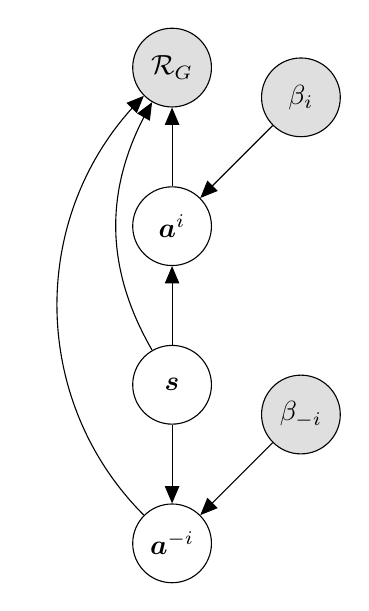
\begin{tikzpicture}[latent/.append style={minimum size=1.0cm}]
        \node[obs] (o) {$\mathcal{R}_G$};
        \node[latent, below=of o] (a) {$\boldsymbol{a}^i$};
        \node[latent, below=of a] (s) {$\boldsymbol{s}$};
        \node[latent, below=of s] (a1) {$\boldsymbol{a}^{-i}$};
        
        \node [obs, above right=1.3cm of a] (beta)  {$\beta_i$};
        
        \node [obs, above right=1.3cm of a1] (beta1)  {$\beta_{-i}$};
    
        \edge {s} {a, a1}
        \edge {beta1} {a1}
        \edge {beta} {a}
        \edge {a} {o}
        \path[->]  (a1)  edge   [bend left=45] node {} (o);
        \path[->]  (s)  edge   [bend left=30] node {} (o);
    \end{tikzpicture}
    \label{Balancing-Graphical}
    \end{minipage}%
    \begin{minipage}[t]{0.5\linewidth}
    Graphical model of One-Step of the algorithm defined in  \cite{grau2018balancing}. We can see that in this work, authors doesn't assume optimality of opponent model. Instead, they assume that the action of the opponent is known. Further more, the $\beta$-value is also known to agents and their opponent.
    \end{minipage}
\end{figure}
We can define the variational distribution to be equal to 
\begin{equation}
     q(\boldsymbol{s}, \boldsymbol{a}^i, \boldsymbol{a}^{-i}, \beta_i = \beta_{\text{pl}}, \beta_{-i} = \beta_{\text{op}}) = P(\boldsymbol{s}) \cdot P(\boldsymbol{a}^i | \boldsymbol{s}, \beta_i = \beta_{\text{pl}}) \cdot P(\boldsymbol{a}^{-i} | \boldsymbol{s}, \beta_i = \beta_{\text{op}})
\end{equation}
In which, we define the agent's policy and opponent's policy to be in the form of
\begin{equation}\label{balance-pol-op}
     P(\boldsymbol{a}^i | \boldsymbol{s}, \beta_i = \beta_{\text{pl}}) = \frac{\pi_{\theta}(\boldsymbol{a}^i |\boldsymbol{s})^{\frac{1}{\beta_{\text{pl}}}}}{N_{\text{pl}}(\boldsymbol{s})} = \frac{e^{\frac{1}{\beta}_{\text{pl}} \log \pi_{\theta}(\boldsymbol{a}^i | s)} }{N_{\text{pl}}(s)} \quad P(\boldsymbol{a}^{-i} | \boldsymbol{s}, \beta_i = \beta_{\text{pl}}) = \frac{\rho_{\phi}(\boldsymbol{a}^{-i} |\boldsymbol{s})^{\frac{1}{\beta_{\text{op}}}}}{N_{\text{op}}(\boldsymbol{s})}
\end{equation}
Similarly, the joint probability distribution that we want to estimate is defined to be 
\begin{equation}
    \begin{aligned}
        P(\boldsymbol{s}, \boldsymbol{a}^i, \boldsymbol{a}^{-i}, \mathcal{O} = 1, \beta_i = \beta_{\text{pl}}, \beta_{-i} = \beta_{\text{op}}) = &P(\mathcal{R}_G | \boldsymbol{s}, \boldsymbol{a}^i, \boldsymbol{a}^{-i})\cdot P(\bold{s}) \cdot \\
        &P_{\text{prior}}(\boldsymbol{a}^i | \boldsymbol{s}, \beta_i = \beta_{\text{pl}}) \cdot P_{\text{prior}}(\boldsymbol{a}^{-i} | \boldsymbol{s}, \beta_i = \beta_{\text{opp}}) \cdot \\
        &P(\beta_i) \cdot P(\beta_{-i})
    \end{aligned}
\end{equation}
In which, the priors for agent and opponent is defined to be (slightly abusing a notation)
\begin{equation}
    P_{\text{prior}}(\boldsymbol{a}^i | \boldsymbol{s}, \beta_i = \beta_{\text{pl}}) = \frac{P_{\text{prior}}(\boldsymbol{a}^i | \boldsymbol{s})^{\frac{1}{\beta_{\text{pl}}}}}{M_{\text{pl}}(\boldsymbol{s})} \quad \quad P_{\text{prior}}(\boldsymbol{a}^{-i} | \boldsymbol{s}, \beta_i = \beta_{\text{op}}) = \frac{P_{\text{prior}}(\boldsymbol{a}^{-i} | \boldsymbol{s})^{\frac{1}{\beta_{\text{op}}}}}{M_{\text{op}}(\boldsymbol{s})}
\end{equation}
The normalizing factor is defined in the form of 
\begin{equation}
    \int P_{\xi}(x | y)^{\alpha} \ dy \quad \text{ or } \quad \int \exp\left(\frac{1}{\alpha} \log P_{\xi}(y)\right) \ dy 
\end{equation}
The game reward for agents is defined to be 
\begin{equation}
    P(\mathcal{R}_G | \boldsymbol{s}, \boldsymbol{a}^i, \boldsymbol{a}^{-i}) = \exp \left( \mathcal{R}_{G}(\boldsymbol{s}, \boldsymbol{a}^i, \boldsymbol{a}^{-i}) \right)
\end{equation}
Doing the variational approximation, we have that 
\begin{equation}
    \begin{aligned}
        &\begin{aligned}[t]
            \mathbb{E}_{(\boldsymbol{s}, \boldsymbol{a}^i, \boldsymbol{a}^{-i}) \sim q(\boldsymbol{s}, \boldsymbol{a}^i, \boldsymbol{a}^{-i}, \beta_i = \beta_{\text{pl}}, \beta_{-i} = \beta_{\text{op}})}\Big[ &\log q(\boldsymbol{s}, \boldsymbol{a}^i, \boldsymbol{a}^{-i}, \beta_i = \beta_{\text{pl}}, \beta_{-i} = \beta_{\text{op}}) \\
            &- \log P(\boldsymbol{s}, \boldsymbol{a}^i, \boldsymbol{a}^{-i}, \mathcal{O} = 1, \beta_i = \beta_{\text{pl}}, \beta_{-i} = \beta_{\text{op}}) \Big]
        \end{aligned} \\
        &= \begin{aligned}[t]
            \mathbb{E}\Bigg[\cancel{\log P(\boldsymbol{s})} &+\log \left[\frac{\pi_{\theta}(\boldsymbol{a}^i |\boldsymbol{s})^{\frac{1}{\beta_{\text{pl}}}}}{N_{\text{pl}}(\boldsymbol{s})}\right] + \log \left[ \frac{\rho_{\phi}(\boldsymbol{a}^{-i} |\boldsymbol{s})^{\frac{1}{\beta_{\text{op}}}}}{N_{\text{op}}(\boldsymbol{s})} \right] \\
            &- \log\left[\frac{P_{\text{prior}}(\boldsymbol{a}^i | \boldsymbol{s})^{\frac{1}{\beta_{\text{pl}}}}}{M_{\text{pl}}(\boldsymbol{s})}\right] -\log\left[ \frac{P_{\text{prior}}(\boldsymbol{a}^{-i} |\boldsymbol{s})^{\frac{1}{\beta_{\text{op}}}}}{M_{\text{op}}(\boldsymbol{s})}\right] \\
            &- \log P(\mathcal{R}_G | \boldsymbol{s}, \boldsymbol{a}^i, \boldsymbol{a}^{-i})-\cancel{\log P(\boldsymbol{s})}  \\
            &- \cancelto{0}{\log P(\beta_i)} - \cancelto{0}{\log P(\beta_{-i})}\Bigg] 
        \end{aligned}  \\
        &=\begin{aligned}[t]
            \mathbb{E}\Bigg[\frac{1}{\beta_{\text{pl}}}&\log \pi_{\theta}(\boldsymbol{a}^i |\boldsymbol{s}) - \log N_{\text{pl}}(\boldsymbol{s}) + \frac{1}{\beta_{\text{op}}}\rho_{\phi}(\boldsymbol{a}^{-i} |\boldsymbol{s}) - \log N_{\text{op}}(\boldsymbol{s}) \\
            &- \frac{1}{\beta_{\text{pl}}}\log P_{\text{prior}}(\boldsymbol{a}^i | \boldsymbol{s}) + \log M_{\text{pl}}(\boldsymbol{s})  -\log \frac{1}{\beta_{\text{op}}}P_{\text{prior}}(\boldsymbol{a}^{-i} |\boldsymbol{s}) + \log M_{\text{op}}(\boldsymbol{s}) - \mathcal{R}_{G}(\boldsymbol{s}, \boldsymbol{a}^i, \boldsymbol{a}^{-i})\Bigg] 
        \end{aligned} \\
        &=\begin{aligned}[t]
            \mathbb{E}\Bigg[ - \mathcal{R}_{G}(\boldsymbol{s}, \boldsymbol{a}^i, \boldsymbol{a}^{-i}) + \frac{1}{\beta_{\text{pl}}}\left(\log \frac{\pi_{\theta}(\boldsymbol{a}^i |\boldsymbol{s})}{P_{\text{prior}}(\boldsymbol{a}^i | \boldsymbol{s})}\right) + \frac{1}{\beta_{\text{op}}} \left(\log \frac{\rho_{\phi}(\boldsymbol{a}^{-i} |\boldsymbol{s})}{P_{\text{prior}}(\boldsymbol{a}^{-i} |\boldsymbol{s})}\right) + \log\left(\frac{M_{\text{pl}}(\boldsymbol{s})M_{\text{op}}(\boldsymbol{s})}{N_{\text{pl}}(\boldsymbol{s})N_{\text{op}}(\boldsymbol{s})}\right) \Bigg]
        \end{aligned}
    \end{aligned}
\end{equation}
This is equivalent to maximizing the following objective
\begin{equation}
    \mathbb{E}\Bigg[ \mathcal{R}_{G}(\boldsymbol{s}, \boldsymbol{a}^i, \boldsymbol{a}^{-i}) - \frac{1}{\beta_{\text{pl}}}\left(\log \frac{\pi_{\theta}(\boldsymbol{a}^i |\boldsymbol{s})}{P_{\text{prior}}(\boldsymbol{a}^i | \boldsymbol{s})}\right) - \frac{1}{\beta_{\text{op}}} \left(\log \frac{\rho_{\phi}(\boldsymbol{a}^{-i} |\boldsymbol{s})}{P_{\text{prior}}(\boldsymbol{a}^{-i} |\boldsymbol{s})}\right) - \log\left(\frac{M_{\text{pl}}(\boldsymbol{s})M_{\text{op}}(\boldsymbol{s})}{N_{\text{pl}}(\boldsymbol{s})N_{\text{op}}(\boldsymbol{s})}\right) \Bigg]
\end{equation}
Noted that the expectation is based on the variational distribution, and thus the agent's policy and opponent's policy is based on the form of \ref{balance-pol-op}. Although the final equation is somewhat undesirable, this is an alternative to  Lagrange multiplier proposed in \cite{grau2018balancing}.

% \section{PR2 \cite{wen2019probabilistic}}
% For PR2, the graphical model is similar to \cite{tian2019regularized}, therefore, the derivation is similar. 

\section{ROMMEO \cite{tian2019regularized} x Balance Soft Q-Learning \cite{grau2018balancing}}

Now we can merge the idea of both model into one, whereby this will enable \cite{tian2019regularized} to be able to work within the zero-sum domain with known other agent's rationality and intention.

\section{Dealing with Unknown $\beta_{-i}$}
Now we would like to extend the merge of ROMMEO \cite{tian2019regularized} and Balance Soft Q-Learning \cite{grau2018balancing}, in which, the agent have some belief over the rationality and intention of other agent. This must be employed some inverse reinforcement learning in multi-agent domain, which is extensively studied. Furthermore, we would like to assert that  \cite{grau2018balancing} has ,also, done some work on estimating $\beta_{-i}$ via maximum likelihood.

\begin{figure}[ht]
    \begin{minipage}[t]{0.5\linewidth}
    \centering
    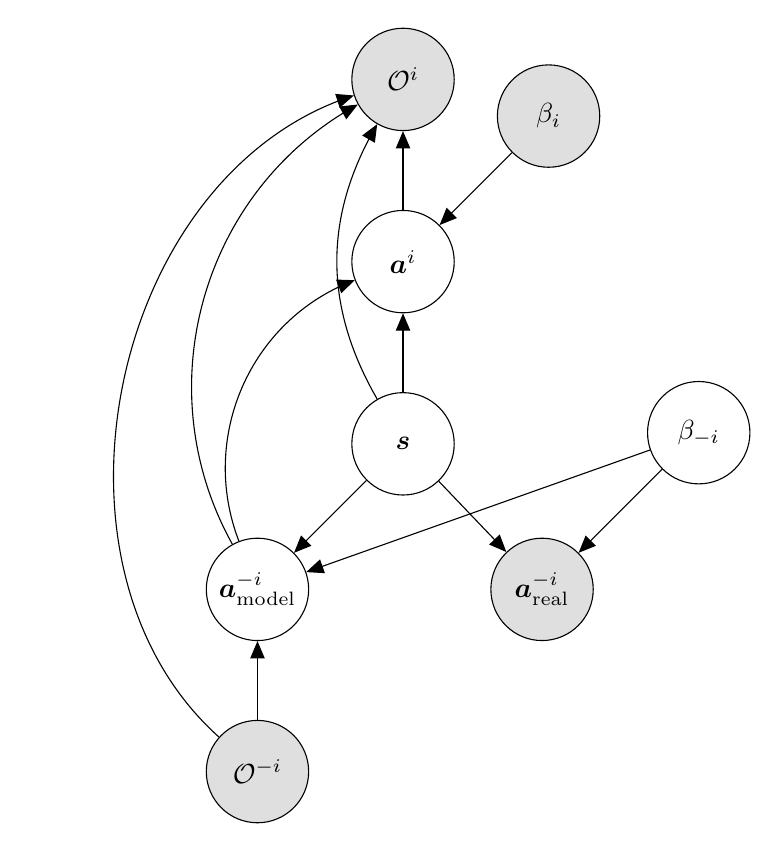
\begin{tikzpicture}[latent/.append style={minimum size=1.3cm}]
        \node[obs] (o) {$\mathcal{O}^i$};
        \node[latent, below=of o] (a) {$\boldsymbol{a}^i$};
        \node[latent, below=of a] (s) {$\boldsymbol{s}$};
        \node[latent, below left=1.3cm of s] (a1model) {$\boldsymbol{a}^{-i}_{\text{model}}$};
        
        \node[obs, right=2.3cm of a1model] (a1real) {$\boldsymbol{a}^{-i}_{\text{real}}$};
        \node [obs, above right=1.3cm of a] (beta)  {$\beta_i$};
        \node [latent, above right=1.5cm of a1real] (beta1)  {$\beta_{-i}$};
        \node[obs, below=of a1model] (o1) {$\mathcal{O}^{-i}$};
    
        \edge {s} {a, a1model, a1real}
        \edge {beta1} {a1model, a1real}
        \edge {beta} {a}
        \edge {a} {o}
        \edge {o1} {a1model}
        \path[->]  (a1model)  edge   [bend left=45] node {} (o);
        \path[->]  (s)  edge   [bend left=30] node {} (o);
        \path[->]  (o1)  edge   [bend left=60] node {} (o);
        \path[->]  (a1model)  edge   [bend left=45] node {} (a);
    \end{tikzpicture}
    \label{Balancing-Graphical}
    \end{minipage}%
    \begin{minipage}[t]{0.5\linewidth}
    We will model the belief over $\beta_{-i}$, which influences opponent's action, and we will use this value to construct perfect opponent model, such that agent can best response to. \Phu{It would be interesting if we assume that the real action of other agents based on our action (which isn't the case in one step game)}
    \end{minipage}
\end{figure}

\blindtext

\section{Probabilistic Model For General Sum Game}
Most of the models till now are all based on the centralized game rewards of all agents, while in \cite{grau2018balancing} the type of the game is based on the sign of $\beta_{-i}$, which reflects how the opponent agent itself react based on its perspective of the game reward.

This carves the way for us by defining $\beta_{-i}(\boldsymbol{s}, \boldsymbol{a}^i, \boldsymbol{a}^{-i})$ to be varied according to all agents actions and state. \Phu{VERY VERY WEIRD INITIAL IDEA. This would be a disaster for defining the normalizing factor ?}, notably 
\begin{equation}
    \beta_{-i}(\boldsymbol{s}, \boldsymbol{a}^i, \boldsymbol{a}^{-i}) = \frac{R_{-i}(\boldsymbol{s}, \boldsymbol{a}^i, \boldsymbol{a}^{-i})}{R_i(\boldsymbol{s}, \boldsymbol{a}^i, \boldsymbol{a}^{-i})}
\end{equation}

\chapter{Experiments}

\chapter{Extensions/Future Work (If have time)}
\section{Extension to N-Agents}

\section{Agent with learnt prior (mutual information maximization)}

\section{Belief Over $\beta$s}

\section{General sum game -- learned Q-function}

\chapter{Conclusion}
\begin{itemize}
    \item Pure Nash Strategy from VIREL
    \item Graph Neural Network 
    \item Unified View. 
    \item Modeling Belief 
\end{itemize}

% \appendix

\bibliographystyle{alpha}
\bibliography{bibilography}

\chapter{Overview of ELBO, EM and Variational Inference}
ELBO or Evidence Lower Bound Objective is one of the most interesting and fruitful objective functions. Its applications span in the from probabilistic generative models \cite{kingma2013auto} to reinforcement learning \cite{levine2018reinforcement}. This section will provides common "pattern" for deriving ELBO, which ultimately leads to Expectation Maximization algorithm, variational inference and variational auto-encoder \cite{kingma2013auto}  \Phu{Cite EM Cite VI add more examples}

Suppose we would like to maximize the probability of generating data point $\boldsymbol{X}$ given the parameter $\boldsymbol{\theta}$. We can assume there exists a latent variable $\boldsymbol{z}$ that generates this data point. Writing it as (assuming $q(\boldsymbol{z})$ is an arbitrary distribution over $\boldsymbol{z}$)

\begin{equation}
    \begin{aligned}
         \log P(\boldsymbol{X} | \boldsymbol{\theta}) &= \int P(\boldsymbol{X}, \boldsymbol{z} | \boldsymbol{\theta}) \ d\boldsymbol{z} \\
         &= \log \int P(\boldsymbol{X}, \boldsymbol{z}) \frac{q(\boldsymbol{z})}{q(\boldsymbol{z})} \ d \boldsymbol{z} \\
         &= \log \mathbb{E}_{\boldsymbol{z} \sim q(\boldsymbol{z})} \left[ \frac{P(\boldsymbol{X}, \boldsymbol{z} | \boldsymbol{\theta})}{q(\boldsymbol{z})} \right] \\
         &\ge \mathbb{E}_{\boldsymbol{z} \sim q(\boldsymbol{z})} \left[ \log\frac{P(\boldsymbol{X}, \boldsymbol{z} | \boldsymbol{\theta})}{q(\boldsymbol{z})} \right]
    \end{aligned}
\end{equation}
The inequality came from Jensen's inequality, hence we arrived at ELBO. The difference between ELBO and $\log P(\boldsymbol{X} |\boldsymbol{\theta})$ is equal to 

\begin{equation}
    \begin{aligned}
        \log P(\boldsymbol{X} |\boldsymbol{\theta}) - &\mathbb{E}_{\boldsymbol{z} \sim p(\boldsymbol{z})} \left[ \log\frac{P(\boldsymbol{X}, \boldsymbol{z} | \boldsymbol{\theta})}{q(\boldsymbol{z})} \right] \\
        &= \log P(\boldsymbol{X} |\boldsymbol{\theta}) - \mathbb{E}_{\boldsymbol{z} \sim q(\boldsymbol{z})}\big[ \log P(\boldsymbol{X}, \boldsymbol{z} | \boldsymbol{\theta}) \big] + \mathbb{E}_{\boldsymbol{z} \sim q(\boldsymbol{z})} \big[ \log q(\boldsymbol{z}) \big]  \\ 
        &= \cancel{\log P(\boldsymbol{X} |\boldsymbol{\theta})} - \mathbb{E}_{\boldsymbol{z} \sim q(\boldsymbol{z})}\big[ \log P( \boldsymbol{z} |\boldsymbol{X} , \boldsymbol{\theta}) \big] - \cancel{\mathbb{E}_{\boldsymbol{z} \sim q(\boldsymbol{z})}\big[ \log P( \boldsymbol{X} | \boldsymbol{\theta}) \big]} + \mathbb{E}_{\boldsymbol{z} \sim q(\boldsymbol{z})} \big[ \log q(\boldsymbol{z}) \big] \\ 
        &=  \mathbb{E}_{\boldsymbol{z} \sim q(\boldsymbol{z})} \big[ \log q(\boldsymbol{z}) \big] - \mathbb{E}_{\boldsymbol{z} \sim q(\boldsymbol{z})} \big[ \log P( \boldsymbol{z} |\boldsymbol{X} , \boldsymbol{\theta}) \big] \\
        &= D_{KL} \left( q(\boldsymbol{z}) || P( \boldsymbol{z} |\boldsymbol{X} , \boldsymbol{\theta}) \right)
    \end{aligned}
\end{equation}
This leads to first optimization step of EM algorithm (E-Step), where the goals of this algorithm is maximizes $\log$ probability. We would like to minimizing the "gap" between ELBO and $P(\boldsymbol{x} | \boldsymbol{\theta})$, therefore in E-Step, we set: 

$$
q(\boldsymbol{z}) \leftarrow P( \boldsymbol{z} |\boldsymbol{X} , \boldsymbol{\theta})
$$

So now, we have that ELBO is equal to $P(\boldsymbol{x} | \boldsymbol{\theta})$, which we now proceeded to maximizing ELBO based on $\theta$, which is equal to optimizing the following objective. 

\begin{equation}
    \arg\max_{\boldsymbol{\theta}} \mathbb{E}_{\boldsymbol{z} \sim q(\boldsymbol{z})}\big[\log P(\boldsymbol{X}, \boldsymbol{z} | \theta)\big]
\end{equation}
We call this step, M-Step. The limitation of EM algorithm lies within in E-Step, suppose, we can't even compute $P( \boldsymbol{z} |\boldsymbol{X} , \boldsymbol{\theta})$ then we have to minimizing the KL distance with respect to parameterized $\phi$ of $q(\boldsymbol{z} | \boldsymbol{X}, \boldsymbol{\phi})$, instead: 

\begin{equation}
    D_{KL}(q(\boldsymbol{z}| \boldsymbol{X}, \boldsymbol{\phi}) || P( \boldsymbol{z} |\boldsymbol{X} , \boldsymbol{\theta}) )
\end{equation}
Which can be shown to be equal to minimizing ELBO for both parameters $\boldsymbol{\phi}, \boldsymbol{\theta}$
\begin{equation}
    \begin{aligned}
        D_{KL}(q(\boldsymbol{z}| \boldsymbol{X}, \boldsymbol{\phi}) || P( \boldsymbol{z} |\boldsymbol{X} , \boldsymbol{\theta}) ) &= \mathbb{E}_{\boldsymbol{z} \sim q(\boldsymbol{z} | \boldsymbol{X}, \boldsymbol{\phi})} \left[ \log \frac{q(\boldsymbol{z} | \boldsymbol{X}, \boldsymbol{\phi})}{P(\boldsymbol{z} | \boldsymbol{X}, \boldsymbol{\theta})} \right] \quad \text{ where } P(\boldsymbol{z} | \boldsymbol{X}, \boldsymbol{\theta}) = \frac{P(\boldsymbol{X} | \boldsymbol{z}, \boldsymbol{\theta}) P(\boldsymbol{z})}{P(\boldsymbol{X} | \boldsymbol{\theta})} \\ 
        &= \mathbb{E}_{\boldsymbol{z} \sim q(\boldsymbol{z} | \boldsymbol{X}, \boldsymbol{\phi})} \left[ \log \frac{q(\boldsymbol{z} | \boldsymbol{X}, \boldsymbol{\phi}) P(\boldsymbol{X} | \boldsymbol{\theta})}{P(\boldsymbol{X} | \boldsymbol{z}, \boldsymbol{\theta}) P(\boldsymbol{z})} \right] \\ 
        &= \underbrace{\mathbb{E}_{\boldsymbol{z} \sim q(\boldsymbol{z} | \boldsymbol{X}, \boldsymbol{\phi})} \left[ \log \frac{q(\boldsymbol{z} | \boldsymbol{X}, \boldsymbol{\phi})}{P(\boldsymbol{X} | \boldsymbol{z}, \boldsymbol{\theta}) P(\boldsymbol{z})} \right]}_{\text{ELBO}} + \mathbb{E}_{\boldsymbol{z} \sim q(\boldsymbol{z} | \boldsymbol{X}, \boldsymbol{\phi})} \left[ \log P(\boldsymbol{X} | \boldsymbol{\theta}) \right]  \\ 
        &= -\mathbb{E}_{\boldsymbol{z} \sim q(\boldsymbol{z} | \boldsymbol{X}, \boldsymbol{\phi})} \left[ \log P(\boldsymbol{X} | \boldsymbol{z}, \boldsymbol{\theta}) \right] + \mathbb{E}_{\boldsymbol{z} \sim q(\boldsymbol{z} | \boldsymbol{X}, \boldsymbol{\phi})} \left[ \log \frac{q(\boldsymbol{z} | \boldsymbol{X}, \boldsymbol{\phi})}{P(\boldsymbol{z})} \right] + \text{const} \\ 
        &= -\mathbb{E}_{\boldsymbol{z} \sim q(\boldsymbol{z} | \boldsymbol{X}, \boldsymbol{\phi})} \left[ \log P(\boldsymbol{X} | \boldsymbol{z}, \boldsymbol{\theta}) \right] + D_{KL}(q(\boldsymbol{z} | \boldsymbol{X}, \boldsymbol{\phi}) || P(\boldsymbol{z})) + \text{const}
    \end{aligned}
\end{equation}
Now we can also arrived at the ELBO objective. We can interpreted optimizing ELBO with respect to $\phi, \theta$ as EM algorithm where optimizing with respect to $\phi$ is an E-Step and optimizing with respect to $\theta$ is an M-Step. This is also used as optimizing objective in Variational Auto Encoder \cite{kingma2013auto}, where we denote $q(\boldsymbol{z} | \boldsymbol{X}, \boldsymbol{\phi})$ as an encoder and $P(\boldsymbol{X} | \boldsymbol{z}, \boldsymbol{\theta})$ as a decoder




% \chapter{Soft-Q Learning Objective from Probabilistic Interpretation of Reinforcement Learning}
% In the survey \cite{levine2018reinforcement}, the authors provided probabilistic interpretation of reinforcement learning, however, they assume the prior over actions to be uniform. Similarly \cite{grau2018soft} briefly provide and derive objective with explicit prior over actions. In this section, we will go in depth on how to derived such an objective.

We start with assuming a hidden variables $\boldsymbol{a}_{1:T}$ and $\boldsymbol{s}_{1:T}$, where the observed variable to be the optimality $\mathcal{O}_{1:T}$. Given by the following graphical models.

\begin{figure}[!h]
  \tikz{
     \node[obs] (o1) {$\mathcal{O}_1$};
     \node[latent, below=of o1] (a1) {$\bold{a}_1$};
     \node[latent, below=of a1] (s1) {$\bold{s}_1$};
     
     \node[obs, right=of o1] (o2) {$\mathcal{O}_2$};
     \node[latent, right=of a1] (a2) {$\bold{a}_2$};
     \node[latent, right=of s1] (s2) {$\bold{s}_2$};
     
     \node[latent, right=of s2] (s3) {$\bold{s}_3$};
     \node[latent, right=of s3] (st) {$\bold{s}_T$};
     \node at ($(s3)!.5!(st)$) {\ldots};
     
     \path[->]  (s1)  edge   [bend left=30] node {} (o1);
     \edge {a1} {o1}  
     
     \path[->]  (s2)  edge   [bend left=30] node {} (o2);
     \edge {s1, a1} {s2}
     \edge {a2} {o2}
     
     \edge {s2, a2} {s3}
    %  \node[latent,above=of o, xshift=-1cm,fill] (y) {$y$}; 
    %  \node[latent,above=of o,xshift=1cm] (z) {$z$};
    %  \edge {y,z} {o}  
 }
\end{figure}

\Phu{Check this out}
Where we defined the optimality $\mathcal{O}_{1:T}$ to be (Assuming $r$ to always be positive)
\begin{equation}
    P(\mathcal{O}_{t} = 1 | \boldsymbol{s}_{t}, \boldsymbol{a}_{t}) = \frac{\exp\left(\beta \cdot r(\boldsymbol{s}_{t}, \boldsymbol{a}_{t})\right)}{\int \exp(\beta \cdot r(\boldsymbol{s}_{t}, \boldsymbol{a}_{t})) \ d\boldsymbol{s}_{t} d\boldsymbol{a}_{t}}
\end{equation}
And we can see that 
\begin{equation}
    P(\mathcal{O}_{1:T} | \boldsymbol{s}_{1:T}, \boldsymbol{a}_{1:T}) \propto \exp \left( \beta \sum^T_{t=1} r(s_t, a_t) \right)
\end{equation}
Since each optimality variables are conditional independent for each time step. 

We would like to find approximated posterior distribution $q$, which we defined it by probabilistic graphical model as
\begin{figure}[!h]
  \tikz{
     \node[latent] (a1) {$\bold{a}_1$};
     \node[latent, below=of a1] (s1) {$\bold{s}_1$};
     
     \node[latent, right=of a1] (a2) {$\bold{a}_2$};
     \node[latent, right=of s1] (s2) {$\bold{s}_2$};
     
     \node[latent, right=of s2] (s3) {$\bold{s}_3$};
     \node[latent, right=of s3] (st) {$\bold{s}_T$};
     \node at ($(s3)!.5!(st)$) {\ldots};
     
     \edge {s1} {a1}  
     \edge {s1, a1} {s2}
     \edge {s2} {a2}
     
     \edge {s2, a2} {s3}
    %  \node[latent,above=of o, xshift=-1cm,fill] (y) {$y$}; 
    %  \node[latent,above=of o,xshift=1cm] (z) {$z$};
    %  \edge {y,z} {o}  
 }
\end{figure}

The joint probability distribution of $q(\boldsymbol{s}_{1:T}, \boldsymbol{a}_{1:T})$ to be 
\begin{equation}
    q(\boldsymbol{s}_{1:T}, \boldsymbol{a}_{1:T}) = P(\boldsymbol{s}_1)\prod^T_{t=1} P(\boldsymbol{s}_{t+1} | \boldsymbol{s}_t, \boldsymbol{a}_t) \pi_{\theta}(\boldsymbol{a}_t | \boldsymbol{s}_t)
\end{equation}
Now we can minimize the KL-Divergence to perform approximate variational inference.
\begin{equation}
        D_{KL} \Big[ q(\boldsymbol{s}_{1:T}, \boldsymbol{a}_{1:T}) \Big\lvert\Big\rvert P(\boldsymbol{s}_{1:T}, \boldsymbol{a}_{1:T} | \mathcal{O}_{1:T} = 1) \Big] = D_{KL} \left[ q(\boldsymbol{s}_{1:T}, \boldsymbol{a}_{1:T}) \Bigg\lvert\Bigg\rvert \frac{P(\mathcal{O}_{1:T} | \boldsymbol{s}_{1:T}, \boldsymbol{a}_{1:T}) P_{\text{prior}} (\boldsymbol{s}_{1:T}, \boldsymbol{a}_{1:T}) }{P(\mathcal{O}_{1:T})} \right]
\end{equation}
The $P_{\text{prior}}$ is defined to be 
\begin{equation}
    P_{\text{prior}}(\boldsymbol{s}_{1:T}, \boldsymbol{a}_{1:T}) = P(\boldsymbol{s}_1)\prod^T_{t=1} P(\boldsymbol{s}_{t+1} | \boldsymbol{s}_t, \boldsymbol{a}_t) \pi_{\text{prior}}(\boldsymbol{a}_t | \boldsymbol{s}_t)
\end{equation}
Which the evaluation of KL-Divergence yields optimizing the following objective
\begin{equation}
    \begin{aligned}
        \mathbb{E}_{(\boldsymbol{s}_{1:T}, \boldsymbol{a}_{1:T}) \sim q(\boldsymbol{s}_{1:T}, \boldsymbol{a}_{1:T})} &\left[ \log q(\boldsymbol{s}_{1:T}, \boldsymbol{a}_{1:T}) \right] -  \mathbb{E}_{(\boldsymbol{s}_{1:T}, \boldsymbol{a}_{1:T}) \sim q(\boldsymbol{s}_{1:T}, \boldsymbol{a}_{1:T})} \left[ \log \frac{P(\mathcal{O}_{1:T} | \boldsymbol{s}_{1:T}, \boldsymbol{a}_{1:T}) P_{\text{prior}} (\boldsymbol{s}_{1:T}, \boldsymbol{a}_{1:T}) }{P(\mathcal{O}_{1:T})} \right] \\ 
        &= \ \begin{aligned}[t]
           &\mathbb{E}_{(\boldsymbol{s}_{1:T}, \boldsymbol{a}_{1:T}) \sim q(\boldsymbol{s}_{1:T}, \boldsymbol{a}_{1:T})} \left[ \log \left[ P(\boldsymbol{s}_1) \prod^T_{t=1} P(\boldsymbol{s}_{t+1} | \boldsymbol{s}_t, \boldsymbol{a}_t) \pi_{\theta}(\boldsymbol{a}_t | \boldsymbol{s}_t) \right] \right] \\
            &- \mathbb{E}_{(\boldsymbol{s}_{1:T}, \boldsymbol{a}_{1:T}) \sim q(\boldsymbol{s}_{1:T}, \boldsymbol{a}_{1:T})} \big[ \log P(\mathcal{O}_{1:T} | \boldsymbol{s}_{1:T}, \boldsymbol{a}_{1:T}) \big] \\ 
            &- \mathbb{E}_{(\boldsymbol{s}_{1:T}, \boldsymbol{a}_{1:T}) \sim q(\boldsymbol{s}_{1:T}, \boldsymbol{a}_{1:T})} \left[ \log \left[ P(\boldsymbol{s}_1) \prod^T_{t=1} P(\boldsymbol{s}_{t+1} | \boldsymbol{s}_t, \boldsymbol{a}_t) \pi_{\text{prior}}(\boldsymbol{a}_t | \boldsymbol{s}_t) \right] \right] 
        \end{aligned} \\
        &= \begin{aligned}[t]
            &\mathbb{E}_{(\boldsymbol{s}_{1:T}, \boldsymbol{a}_{1:T}) \sim q(\boldsymbol{s}_{1:T}, \boldsymbol{a}_{1:T})} \left[ \log P(\boldsymbol{s}_1) + \sum^T_{t=1} \log P(\boldsymbol{s}_{t+1} | \boldsymbol{s}_t, \boldsymbol{a}_t) + \log \pi_{\theta}(\boldsymbol{a}_t | \boldsymbol{s}_t) \right] \\
            &- \mathbb{E}_{(\boldsymbol{s}_{1:T}, \boldsymbol{a}_{1:T}) \sim q(\boldsymbol{s}_{1:T}, \boldsymbol{a}_{1:T})} \left[ \lambda \sum^T_{t=1} r(\boldsymbol{s}_t, \boldsymbol{a}_t) \right] \\
            &- \mathbb{E}_{(\boldsymbol{s}_{1:T}, \boldsymbol{a}_{1:T}) \sim q(\boldsymbol{s}_{1:T}, \boldsymbol{a}_{1:T})} \left[ \log P(\boldsymbol{s}_1) + \sum^T_{t=1} \log P(\boldsymbol{s}_{t+1} | \boldsymbol{s}_t, \boldsymbol{a}_t) + \log \pi_{\text{prior}}(\boldsymbol{a}_t | \boldsymbol{s}_t) \right]
        \end{aligned} \\ 
        &= \begin{aligned}[t]
            &-\mathbb{E}_{(\boldsymbol{s}_{1:T}, \boldsymbol{a}_{1:T}) \sim q(\boldsymbol{s}_{1:T}, \boldsymbol{a}_{1:T})} \left[\lambda \sum^T_{t=1}  r(\boldsymbol{s}_t, \boldsymbol{a}_t) \right] \\
            &+ \mathbb{E}_{(\boldsymbol{s}_{1:T}, \boldsymbol{a}_{1:T}) \sim q(\boldsymbol{s}_{1:T}, \boldsymbol{a}_{1:T})} \left[ \sum^T_{t=1} \log \pi_{\theta}(\boldsymbol{a}_t | \boldsymbol{s}_t) - \log \pi_{\text{prior}}(\boldsymbol{a}_t | \boldsymbol{s}_t) \right]
        \end{aligned}
    \end{aligned}
\end{equation}

The object we have maximizes becomes:
\begin{equation}
    \lambda \mathbb{E}_{(\boldsymbol{s}_{1:T}, \boldsymbol{a}_{1:T}) \sim q(\boldsymbol{s}_{1:T}, \boldsymbol{a}_{1:T})} \left[\sum^T_{t=1}  r(\boldsymbol{s}_t, \boldsymbol{a}_t) \right] - \sum^T_{t=1} D_{KL}\Big[ \pi_{\theta} (\boldsymbol{a}_t | \boldsymbol{s}_t) \Big|\Big| \pi_{\text{prior}} (\boldsymbol{a}_t | \boldsymbol{s}_t) \Big]
\end{equation}
Noted that if the $\pi_{\text{prior}}$ is uniform distribution, then the objective becomes maximum entropy reinforcement learning.



% \chapter{ROMMEO\cite{tian2019regularized}}\label{ROMMEOFull}
% \begin{figure}[ht]
    \begin{minipage}[t]{0.5\linewidth}
    \centering
    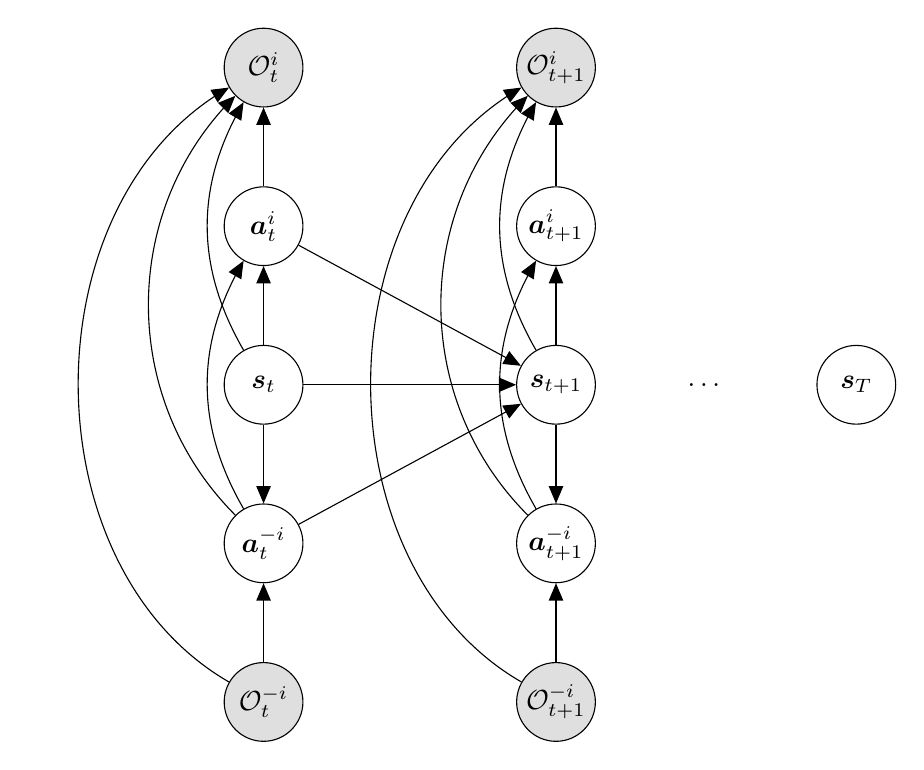
\begin{tikzpicture}[latent/.append style={minimum size=1.0cm}]
        \node[obs] (o) {$\mathcal{O}^i_t$};
        \node[latent, below=of o] (a) {$\boldsymbol{a}^i_t$};
        \node[latent, below=of a] (s) {$\boldsymbol{s}_t$};
        \node[latent, below=of s] (a1) {$\boldsymbol{a}^{-i}_t$};
        \node[obs, below=of a1] (o1) {$\mathcal{O}^{-i}_t$};
        
        \node[obs, right=of o] (o2) [right=2.7cm of o] {$\mathcal{O}^i_{t+1}$};
        \node[latent, right=of s] (s2) [right=2.7cm of s] {$\boldsymbol{s}_{t+1}$};
        \node[latent, right=of a] (a2) [right=2.7cm of a] {$\boldsymbol{a}^i_{t+1}$};
        \node[latent, right=of a1] (a12) [right=2.7cm of a1] {$\boldsymbol{a}^{-i}_{t+1}$};
        \node[obs, right=of o1] (o12) [right=2.7cm of o1] {$\mathcal{O}^{-i}_{t+1}$};
        
        \edge{a, a1, s}{s2}
        
        % \path[->]  (o1)  edge   [bend right=30] node {} (a);
        \edge{o1} {a1}
        \edge {s} {a, a1}
        \edge {a} {o}
        \path[->]  (o1)  edge   [bend left=60] node {} (o);
        \path[->]  (a1)  edge   [bend left=45] node {} (o);
        \path[->]  (a1)  edge   [bend left=30] node {} (a);
        \path[->]  (s)  edge   [bend left=30] node {} (o);
        
        \edge{o12} {a12}
        \edge {s2} {a2, a12}
        \edge {a2} {o2}
        \path[->]  (o12)  edge   [bend left=60] node {} (o2);
        \path[->]  (a12)  edge   [bend left=45] node {} (o2);
        \path[->]  (a12)  edge   [bend left=30] node {} (a2);
        \path[->]  (s2)  edge   [bend left=30] node {} (o2);
        
        \node[latent, right=of s2] (st)[right=2.8cm of s2] {$\boldsymbol{s}_T$};
        
        \node at ($(s2)!.5!(st)$) {\ldots};
        
    \end{tikzpicture}
    \label{ROMMEO-Graphical}
    \end{minipage}%
    \begin{minipage}[t]{0.5\linewidth}
    Graphical model of ROMMEO \cite{tian2019regularized}.Now in the form of stochastic game.
    \end{minipage}
\end{figure}

\end{document}
